\section{Projektive Geometrie}\label{kapitel:ProjektiveGeometrie}
In diesem Kapitel werden wir eine Einführung in die projektive Geometrie geben und an vielen Beispielen demonstrieren, wie projektive Geometrie zur Lösung von Olympiadeaufgaben eingesetzt werden können. Naturgemäß werden wir dafür viel Theorie einführen müssen, wovon euch sehr viel wahrscheinlich neu sein wird. Wenn ihr dieses Kapitel aber einmal verdaut und durchgearbeitet habt, werdet ihr ein ganzes Arsenal an neuen Werkzeugen zur Verfügung haben und ihr werdet Aufgaben mit Leichtigkeit lösen können, die euch vorher sehr schwer gefallen wären.

Die Beispielaufgaben in diesem Kapitel werden direkt aufgelöst, statt dass es wie sonst Tipps und die Lösungen erst am Ende des Heftes gibt. Der Grund dafür ist die Fülle an neuen Methoden, die in diesem Kapitel eingeführt werden. Bevor ihr diese Methoden realistisch selbst anwenden könnt, müsst ihr sie einmal in Aktion gesehen haben. Wenn ihr Lust habt, könnt ihr natürlich trotzdem zuerst selbst an den Aufgaben zu knobeln, bevor ihr weiterlest. Außerdem gibt es am Ende jede Menge Übungsaufgaben zum Vertiefen der Methoden.

Zur projektiven Geometrie gibt es auch ein exzellentes Skript von Jens Reinhold,\footnote{Online verfügbar unter \url{https://drive.google.com/uc?id=1aUdgB5zLRj8MPfwy3r1exr6idfGJR65Z}} an welchem sich dieses Kapitel in großen Teilen orientiert.

\subsection*{Die projektive Ebene}
In vielen geometrischen Konstellationen müssen Spezialfälle betrachtet werden, weil es passieren kann, dass zwei Geraden parallel sind, sodass ein gewünschter Schnittpunkt vielleicht gar nicht existiert. Zum Beispiel gibt es viele Aussagen (und Aufgaben) der Form \enquote{drei Geraden schneiden sich in einem Punkt oder sind paarweise parallel}. Die projektive Ebene ist ein Hilfsmittel, mit dem sich derartige Spezialfälle vermeiden lassen.

Die projektive Ebene entsteht aus der üblichen euklidischen Ebene, indem wir einige \enquote{unendlich weit entfernte Punkte} hinzufügen, sogenannte \emph{Fernpunkte}, die alle auf einer \enquote{unendlich weit entfernten Gerade} liegen, der \emph{Ferngerade}. Konkret stellen wir uns dafür vor, dass jede Gerade~$\ell$ durch einen Fernpunkt~$\infty_\ell$ verläuft. Für zwei Geraden $\ell_1$~und~$\ell_2$ soll genau dann $\infty_{\ell_1}=\infty_{\ell_2}$ gelten, wenn $\ell_1$~und~$\ell_2$ parallel sind. Alle Geraden, die zu einer gegebenen Geraden~$\ell$ parallel sind, schneiden $\ell$ also im Fernpunkt~$\infty_\ell$ (und alle anderen Geraden schneiden~$\ell$ natürlich in einem Nicht-Fernpunkt). Wenn $P$ ein beliebiger Punkt ist, dann definieren wir die \enquote{Gerade~$P\infty_\ell$} als die Parallele zu~$\ell$ durch~$P$. Wenn $\ell_1$ und $\ell_2$ zwei nicht-parallele Geraden sind, das heißt $\infty_{\ell_1}\neq \infty_{\ell_2}$ gilt, dann ist die \enquote{Gerade $\infty_{\ell_1}\infty_{\ell_2}$} genau die Ferngerade.

Es gibt einen Weg, sich die projektive Ebene etwas anschaulicher zu machen. Dazu stellen wir uns vor, dass die euklidische Ebene in Wirklichkeit eine Ebene~$\Sigma$ im Raum ist. Sei $Z$ ein Punkt, der nicht auf~$\Sigma$ liegt. Jedem Punkt~$X$ auf~$\Sigma$ ordnen wir die Gerade~$XZ$ zu und jeder Gerade~$\ell$ in~$\Sigma$ ordnen wir die Ebene~$\Pi_\ell$ zu, die von $\ell$~und~$Z$ aufgespannt wird. Dadurch erhalten wir Abbildungen	
\begin{equation*}
	\begin{aligned}[t]
		\{\text{Punkte auf~$\Sigma$}\}&\longrightarrow \{\text{Geraden durch~$Z$}\}\\
		X&\longmapsto XZ
	\end{aligned}\quad\text{und}\quad 
	\begin{aligned}[t]
		\{\text{Geraden auf~$\Sigma$}\} & \longrightarrow \{\text{Ebenen durch~$Z$}\}\\
		\ell & \longmapsto \Pi_\ell\,.
	\end{aligned}
\end{equation*}
Diese Abbildungen sind injektiv, aber nicht surjektiv. Denn die Geraden durch~$Z$, die zur Ebene~$\Sigma$ parallel sind, können nicht von der Form~$XZ$ für irgendeinen Punkt~$X$ auf~$\Sigma$ sein. Genauso wenig kann die Ebene durch~$Z$, die zu~$\Sigma$ parallel ist, von der Form~$\Pi_\ell$ für irgendeine Gerade~$\ell$ auf~$\Sigma$ sein. Die Fernpunkte und die Ferngerade, die wir in der projektiven Ebene hinzugefügt haben, entsprechen genau den Elementen, die von den obigen Abbildungen nicht getroffen werden.

Die Konvention, Punkte zur Ebene hinzuzufügen, erinnert euch bestimmt an Inversion am Kreis. Allerdings unterscheiden sich die beiden Konstruktionen deutlich: Bei der Inversion haben wir einen einzigen unendlich fernen Punkt~$\infty$ hinzugefügt und Geraden als Kreise durch~$\infty$ betrachtet. Insbesondere schneiden sich beliebige zwei Geraden in~$\infty$. Bei der projektiven Ebene haben wir stattdessen unendlich viele unendlich ferne Punkte hinzugefügt, nämlich einen für jede Klasse von parallelen Geraden. Im Studium werdet ihr erfahren, dass Inversion am Kreis in der \emph{komplex-projektiven Geraden~$\mathbb{CP}^1$} stattfindet (die uns als Ebene erscheint, weil wir uns die komplexen Zahlen~$\mathbb C$ ja selber als Ebene vorstellen), während wir hier mit der \emph{reell-projektiven Ebene~$\mathbb{RP}^2$} arbeiten.

\subsection*{Das Doppelverhältnis}
\begin{definition}
	Seien $A$,~$B$, $C$ und~$D$ vier verschiedene Punkte auf einer Geraden~$\ell$. Das \emph{Doppelverhältnis der Punktepaare $(A,B)$ und $(C,D)$} ist definiert als
	\begin{equation*}
		(A,B;C,D)\coloneqq \frac{AC}{CB}\bigg/\!\frac{AD}{DB}\,,
	\end{equation*}
	wobei alle Streckenlängen als gerichtet zu verstehen sind.
\end{definition}

Ihr könnt euch leicht überlegen, dass das Doppelverhältnis unabhängig von der Wahl der Richtung auf~$BC$ ist (so eine Wahl der Richtung findet ja immer implizit statt, wenn wir mit gerichteten Streckenlängen arbeiten). Das Doppelverhältnis ist außerdem unabhängig von der Reihenfolge der Punktepaare: $(A,B;C,D)=(C,D;A,B)$. Es ist allerdings \emph{nicht} unabhängig von der Reihenfolge der Punkte innerhalb der Punktepaare: Wenn $(A,B;C,D)=\lambda$, dann ist $(B,A;C,D)=1/\lambda$.

Ein wiederkehrendes Motiv in der projektiven Geometrie ist das \emph{Dualitätsprinzip}: Eine Aussage sollte auch dann noch wahr sein, wenn wir \enquote{die Rollen von Punkten und Geraden vertauschen}, das heißt, wenn jeder Punkt durch eine Gerade und jede Gerade durch einen Punkt ersetzt wird, wobei die Verbindungsgerade zweier Punkte durch den Schnittpunkt der entsprechenden Geraden ersetzt wird und umgekehrt. Im letzten Unterkapitel zu Dualität werdet ihr eine Methode kennenlernen, mit der sich dieses Prinzip konkret verwirklichen lässt. Für den Moment nehmen wir das Dualitätsprinzip als Motivation, das Doppelverhältnis nicht nur für Punkte auf einer Geraden, sondern auch für Geraden durch einen Punkt zu definieren. 

\begin{definition}
	Seien $a$,~$b$, $c$ und~$d$ vier verschiedene Geraden, die alle durch den Punkt~$P$ verlaufen. Dann definieren wir das \emph{Doppelverhältnis der Geradenpaare $(a,b)$ und $(c,d)$} als
	\begin{equation*}
		(a,b;c,d)\coloneqq \epsilon\cdot \frac{\sin\winkel(a,c)}{\sin\winkel(c,b)}\bigg/\frac{\sin\winkel (a,d)}{\sin\winkel (d,b)}\,,
	\end{equation*}
	wobei alle Schnittwinkel wie üblich zwischen $0^\circ$~und~$90^\circ$ liegen sollen und das Vorzeichen $\epsilon\in \braces{-1,+1}$ wie folgt definiert ist: Wenn $c$~und~$d$ im gleichen der von $a$~und~$b$ aufgespannten Winkel liegen, dann wählen wir $\epsilon\coloneqq+1$, ansonsten sei $\epsilon\coloneqq-1$.
\end{definition}

\begin{satzmitnamen}[Lemma]
	Seien $A$,~$B$, $C$ und~$D$ vier verschiedene Punkte auf einer Geraden~$\ell$ sind und sei $P$ ein beliebiger Punkt, der nicht auf~$\ell$ liegt. Dann ist %das Doppelverhältnis der Punktepaare $(A,B)$ und $(C,D)$ gleich dem Doppelverhältnis der Geradenpaare $(PA,PB)$ und $(PC,PD)$:
	\begin{equation*}
		\left(A,B;C,D\right)=\left(PA,PB;PC,PD\right)\,.
	\end{equation*}
\end{satzmitnamen}

\begin{proof}
	Es lässt sich leicht nachprüfen, dass $(A,B;C,D)$ und $(PA,PB;PC,PD)$ das gleiche Vorzeichen haben. Wir müssen also nur prüfen, dass auch ihre Beträge übereinstimmen. Die Winkel $\varphi$~und~$\psi$ seien wie in der Skizze definiert. Nach dem Sinussatz in den Dreiecken $ACP$ und $BCP$ gilt $\abs{AC}=\abs{PA}\cdot {\sin\winkel(PA,PC)}/{\sin\varphi}$ und $\abs{CB}=\abs{PB}\cdot {\sin\winkel(PC,PB)}/{\sin\varphi}$. Nach dem Sinussatz in den Dreiecken $ADP$ und $BDP$ gilt $\abs{AD}=\abs{PA}\cdot {\sin\winkel(PA,PD)}/{\sin\psi}$ und $\abs{DB}=\abs{PB}\cdot {\sin\winkel(PD,PB)}/{\sin\psi}$. Durch Einsetzen folgt
	\begin{equation*}
		\frac{\abs{AC}}{\abs{CB}}\bigg/\frac{\abs{AD}}{\abs{DB}}=\frac{\abs{PA}\cdot\sin\winkel(a,c)}{\abs{PB}\cdot \sin\winkel(c,b)}\bigg/\frac{\abs{PA}\cdot\sin\winkel(a,d)}{\abs{PB}\cdot \sin\winkel(d,b)}=\frac{\sin\winkel(a,c)}{\sin\winkel(c,b)}\bigg/\frac{\sin\winkel(a,d)}{\sin\winkel(d,b)}\,,
	\end{equation*}
	also $\abs{(A,B;C,D)}=\abs{(PA,PB;PC,PD)}$, wie gewünscht.
\end{proof}
	\begin{figure}[ht]
	\centering
	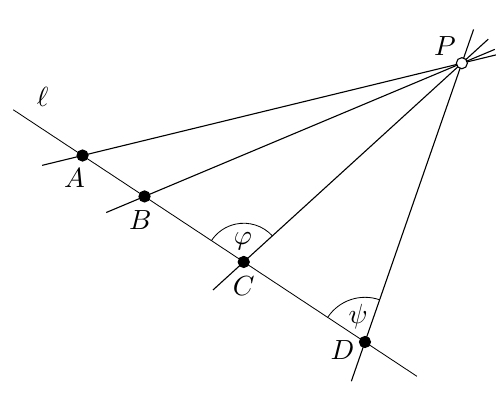
\begin{tikzpicture}[x=0.6cm,y=0.6cm]
		\coordinate (A) at (-1.006,0.404);
		\coordinate (B) at (0.306,-0.462);
		\coordinate (C) at (2.406,-1.849);
		\coordinate (D) at (4.972,-3.543);
		\coordinate (P) at (7.023,2.358);
		\draw [line width=0.3,shorten <=-3em,shorten >=-2.25em] (A) to (D);
		\draw [shorten <=-3ex,shorten >=-1.5em] (P) to (A);
		\draw [shorten <=-3ex,shorten >=-1.5em] (P) to (B);
		\draw [shorten <=-3ex,shorten >=-1.5em] (P) to (C);
		\draw [shorten <=-3ex,shorten >=-1.5em] (P) to (D);
		\draw [line width=0.3, shift={(C)}] (42.34:3.25ex) arc (42.34:146.567:3.25ex);
		\draw [line width=0.3, shift={(D)}] (70.836:3.75ex) arc (70.836:146.567:3.75ex);
		\draw [fill=black] (A) circle (2pt) node[shift={(250:2ex)}] {$A$};
		\draw [fill=black] (B) circle (2pt) node[shift={(260:2ex)}] {$B$};
		\draw [fill=black] (C) circle (2pt) node[shift={(270:2ex)}] {$C$};
		\draw [fill=black] (D) circle (2pt) node[shift={(200:2ex)}] {$D$};
		\draw [fill=white] (P) circle (2pt) node[shift={(135:2ex)}] {$P$};
		\node [shift={(92:1.75ex)}] at (C) {$\varphi$};
		\node [shift={(105:2.25ex)}] at (D) {$\psi$};
		\node at (-1.85,1.65) {$\ell$};
	\end{tikzpicture}
\end{figure}



Das Doppelverhältnis von zwei Punktepaaren auf einer Geraden~$\ell$ lässt sich auch dann definieren, wenn einer der vier Punkte der Fernpunkt~$\infty_\ell$ ist. Wenn zum Beispiel $D=\infty_\ell$ gilt, dann definieren wir $(A,B;C,\infty_\ell)\coloneqq -AC/CB$. Die Logik dahinter ist, dass das Verhältnis $AD/DB$ gegen~$-1$ konvergiert, wenn sich $D$ immer weiter von der Strecke~$\overline{AB}$ entfernt. Wir können das Doppelverhältnis sogar dann definieren, wenn die Gerade~$\ell$ die Ferngerade ist. Wir können nämlich Geraden $a$,~$b$, $c$ und~$d$ wählen, sodass $A=\infty_a$, $B=\infty_b$, $C=\infty_c$ und $D=\infty_d$. Durch Parallelverschiebung können wir erreichen, dass sich $a$,~$b$, $c$ und~$d$ in einem Punkt~$P$ schneiden. Dann definieren wir $(\infty_a,\infty_b;\infty_c,\infty_d)\coloneqq (a,b;c,d)$. Aus dem Lemma folgt, dass diese Definition unabhängig von der Wahl von~$P$ ist. Mit ähnlichen Tricks lässt sich das Doppelverhältnis schließlich auch für Geradenpaare definieren, bei denen eine der Geraden die Ferngerade ist. Durch eine etwas umständliche Fallunterscheidung lässt sich zeigen, dass das vorherige Lemma auch für diese erweiterte Definition des Doppelverhältnisses gültig ist.
% Tien: Da du diese Verallgemeinerung des Doppelverhältnisses auch später im Beweis benutzt, willst du vielleicht sagen, dass das Lemma auch für diesen erweiterten Begriff gilt.

Nachdem wir Doppelverhältnisse für Punktepaare auf einer Geraden und Geradenpaare durch einen Punkt definiert haben, wollen wir zum Schluss noch das Doppelverhältnis für Punktepaare auf einem Kreis definieren.

\begin{definition}
	Seien $A$,~$B$, $C$ und~$D$ vier verschiedene Punkte auf einem Kreis~$\omega$. Das \emph{Doppelverhältnis der Punktepaare $(A,B)$ und $(C,D)$} ist definiert als
	\begin{equation*}
		\left(A,B;C,D\right)\coloneqq \epsilon\cdot \left.\frac{\abs{AC}}{\abs{CB}}\middle/\frac{\abs{AD}}{\abs{DB}}\right.\,,
	\end{equation*}
	wobei wir $\epsilon\coloneqq +1$ wählen, wenn $C$ und $D$ auf dem gleichen der beiden Kreisbögen $\wideparen{AB}$ liegen, sonst wählen wir $\epsilon\coloneqq -1$.
\end{definition}

\begin{satzmitnamen}[Lemma]
	Seien $A$,~$B$, $C$ und~$D$ vier verschiedene Punkte auf einem Kreis~$\omega$ und sei $P$ ein weiterer Punkt auf~$\omega$. Dann ist% das Doppelverhältnis der Punktepaare $(A,B)$ und $(C,D)$ gleich dem Doppelverhältnis der Geradenpaare $(PA,PB)$ und $(PC,PD)$:
	\begin{equation*}
		\left(A,B;C,D\right)=\left(PA,PB;PC,PD\right)
	\end{equation*}
	\embrace{in dem Fall, dass $P$ mit einem der Punkte $A$,~$B$, $C$ oder~$D$ zusammenfällt, interpretieren wir die \enquote{Gerade~$PP$} als die Tangente an~$\omega$ in~$P$}.
\end{satzmitnamen}

\begin{proof}
	Mit einer einfachen Fallunterscheidung lässt sich zeigen, dass die Doppelverhältnisse $(A,B;C,D)$ und $(PA,PB;PC,PD)$ stets das gleiche Vorzeichen haben. Wir müssen also nur prüfen, dass auch ihre Beträge übereinstimmen. Durch Einsetzen der Formeln folgt
	\begin{equation*}
		\frac{\abs{(PA,PB;PC,PD)}}{\abs{(A,B;C,D)}}=\frac{\sin\winkel(PA,PC)}{\abs{AC}}\cdot \frac{\abs{CB}}{\sin\winkel (PC,PB)}\cdot \frac{\abs{AD}}{\sin\winkel(PA,PD)}\cdot \frac{\sin\winkel(PD,PB)}{\abs{DB}}\,.
	\end{equation*}
	Nach dem erweiterten Sinussatz im Dreieck $ACP$ gilt aber $\abs{AC}/\!\sin\winkel(PA,PC)=2r$, wobei $r$ der Radius von~$\omega$ ist.
	% Tien: Vielleicht noch ein Kommentar, dass im Spezialfall, falls P mit einer der vier Punkte zusammenfällt, du den Sehnen-Tangentenwinkelsatz benutzt.
	Analoge Argumente lassen sich auf die anderen Faktoren anwenden. Das Produkt auf der rechten Seite der obigen Gleichung ist also $(2r)^{-1}\cdot (2r)\cdot (2r)\cdot (2r)^{-1}=1$.
	Damit haben wir, wie gewünscht, $\abs{(A,B;C,D)}=\abs{(PA,PB;PC,PD)}$ gezeigt. Das Argument funktioniert auch in dem Fall, dass~$P$ mit einem der Punkte $A$, $B$, $C$ oder $D$ zusammenfällt. In diesem Fall müssen wir den Sehnen-Tangentenwinkelsatz benutzen.
\end{proof}

\subsection*{Projektive Abbildungen}
\begin{definition}
	%Seien $\mathcal X$ und $\mathcal Y$ zwei Mengen von Punkten, die jeweils ein Kreis oder eine Gerade sein können.
	Seien $\mathcal X$~und~$\mathcal Y$ jeweils ein Kreis oder eine Gerade, die wir als Menge von Punkten auffassen.
	% Tien: Ich habe das mal umformuliert.
	Eine Abbildung $\pi\colon \mathcal X\to \mathcal Y$ heißt \emph{projektiv}, wenn sie das Doppelverhältnis erhält, das heißt, wenn für beliebige vier verschiedene Punkte $A,B,C,D\in\mathcal X$ folgendes gilt:
	\begin{equation*}
		(A,B;C,D)=\parens[\big]{\pi(A),\pi(B);\pi(C),\pi(D)}\,.
	\end{equation*}
\end{definition}

\begin{satzmitnamen}[Lemma]
	In den folgenden Fällen ist die Projektion durch einen Punkt eine projektive Abbildung:
	\begin{enumerate}
		\item \label{itm:projAbb:GG}
		Seien $\ell_1$~und~$\ell_2$ zwei Geraden, sei $P$ ein Punkt, der nicht auf~$\ell_1$ liegt, und sei $\pi_1\colon \ell_1\to \ell_2$ die Projektion durch~$P$ von~$\ell_1$ auf~$\ell_2$. Das bedeutet: Für jeden Punkt~$X$ auf~$\ell_1$ ist $\pi_1(X)$ der Schnittpunkt von~$PX$ mit~$\ell_2$; falls $PX$ parallel zu~$\ell_2$ ist definieren wir $\pi_1(X)\coloneqq \infty_{\ell_2}$. Dann ist $\pi_1$ eine projektive Abbildung.
		\item \label{itm:projAbb:GK}
		Sei $\ell$ eine Gerade, sei $\omega$ ein Kreis und sei $P$ ein Punkt auf~$\omega$, der nicht auf~$\ell$ liegt.
		% Tien: Ich bin mir zu 100% sicher, dass P nicht auf \ell liegen darf; habe das korrigiert.
		Sei $\pi_2\colon \ell\to \omega$ die Projektion durch~$P$ von~$\ell$ auf~$\omega$. Das bedeutet: Für jeden Punkt~$X$ auf~$\ell$ ist $\pi_2(X)$ der von~$P$ verschiedene Schnittpunkt von~$PX$ mit~$\omega$; falls $PX$ den Kreis~$\omega$ in~$P$ tangiert, definieren wir $\pi_2(X)\coloneqq P$.
		% und falls $PX$ parallel zu~$\ell$ ist, definieren wir $\pi_2(X)\coloneqq \infty_\ell$.
		% Tien: Der auskommentierte Teilsatz macht keinen Sinn. Es ist doch egal, ob PX parallel zu \ell ist, da es doch immer noch einen Schnittpunkt mit \omega gibt (auch liegt \infty_\ell nicht auf \omega). Was du wahrscheinlich damit meinst ist der Spezialfall für \pi_2'.
		Dann ist $\pi_2$ eine projektive Abbildung. Wenn $\pi_2'\colon\omega\to \ell$ die umgekehrte Projektion durch~$P$ von~$\omega$ auf~$\ell$ ist, dann ist auch $\pi_2'$ projektiv.
		\item \label{itm:projAbb:KK}
		Seien $\omega_1$~und~$\omega_2$ zwei Kreise, die sich in einem Punkt~$P$ schneiden. Sei $\pi_3\colon \omega_1\to \omega_2$ die Projektion durch~$P$ von~$\omega_1$ auf~$\omega_2$. Dann ist $\pi_3$ eine projektive Abbildung.
		% Tien: Willst du vielleicht auch hier Projektion durch einen Punkt erklären, oder gehst du davon aus, das alle Elftklässler das Heft von Klasse 10 kennen?
		\item \label{itm:projAbb:K}
		Sei $\omega$ ein Kreis, sei $P$ ein Punkt, der nicht auf~$\omega$ liegt, und sei $\pi_4\colon \omega\to \omega$ die Projektion durch~$P$ von~$\omega$ auf sich selbst. Das bedeutet: Für jeden Punkt~$X$ auf~$\omega$ ist $\pi_4(X)$ der von~$X$ verschiedene Schnittpunkt von~$PX$ mit~$\omega$; falls $PX$ den Kreis~$\omega$ in~$X$ tangiert, definieren wir $\pi_4(X)\coloneqq X$. Dann ist $\pi_4$ eine projektive Abbildung.
	\end{enumerate}
\end{satzmitnamen}

\begin{proof}
	In jedem der Fälle betrachten wir vier verschiedene Punkte $A$,~$B$, $C$ und~$D$ sowie ihre Bildpunkte $A'$,~$B'$, $C'$ und~$D'$ unter der entsprechenden Abbildung. In den Fällen~\ref{itm:projAbb:GG},~\ref{itm:projAbb:GK} und~\ref{itm:projAbb:KK} können wir die beiden Lemmata aus dem vorherigen Abschnitt anwenden und erhalten sofort
	\begin{equation*}
		(A,B;C,D)=(PA,PB;PC,PD)=(A',B';C',D')\,. 
	\end{equation*}
	Die Abbildungen $\pi_1$,~$\pi_2$, $\pi_2'$ und~$\pi_3$ erhalten also in der Tat das Doppelverhältnis. Im Fall~\ref{itm:projAbb:KK} können wir sogar noch mehr sagen: Die Abbildung~$\pi_3$ ist identisch zur Drehstreckung um den zweiten Schnittpunkt von $\omega_1$~und~$\omega_2$, die $\omega_1$~auf~$\omega_2$ abbildet (falls ihr diesen Fakt noch nicht kanntet, schaut einmal ins Kapitel \emph{\embrace{Dreh-}Streckungen} im Heft für Klasse~10). Und es ist klar, dass Drehstreckungen das Doppelverhältnis erhalten.
	
	\begin{figure}[ht]
		\centering
		\begin{tabularx}{\textwidth}{X c X c X}
			& 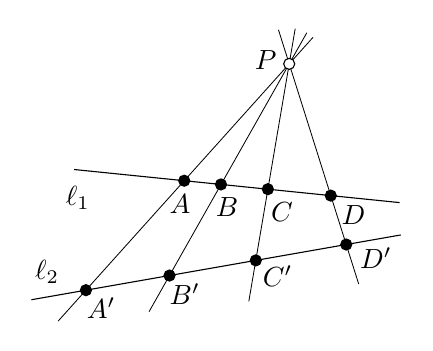
\begin{tikzpicture}[x=0.65cm,y=0.65cm]
				\clip (-0.08,-1.35) rectangle (7.28,4.42);
				\coordinate (P) at (5.03,3.713);
				\coordinate (A) at (2.979,1.43);
				\coordinate (B) at (3.697,1.357);
				\coordinate (C) at (4.613,1.264);
				\coordinate (D) at (5.842,1.139);
				\coordinate (A1) at (1.058,-0.709);
				\coordinate (B1) at (2.691,-0.423);
				\coordinate (C1) at (4.377,-0.127);
				\coordinate (D1) at (6.144,0.183);
				\draw [line width=0.3,shorten <=-3ex,shorten >=-1.5em] (P) to (A1);
				\draw [line width=0.3,shorten <=-3ex,shorten >=-1.5em] (P) to (B1);
				\draw [line width=0.3,shorten <=-3ex,shorten >=-1.5em] (P) to (C1);
				\draw [line width=0.3,shorten <=-3ex,shorten >=-1.5em] (P) to (D1);
				\draw [shorten <=-4em,shorten >=-2.5em] (A) to (D);
				\draw [shorten <=-2em,shorten >=-2em] (A1) to (D1);
				\draw [fill=white] (P) circle (2pt) node[shift={(170:2ex)}] {$P$};
				\draw [fill=black] (A) circle (2pt) node[shift={(260:2ex)}] {$A$};
				\draw [fill=black] (B) circle (2pt) node[shift={(285:2ex)}] {$B$};
				\draw [fill=black] (C) circle (2pt) node[shift={(302:2.25ex)}] {$C$};
				\draw [fill=black] (D) circle (2pt) node[shift={(320:2.5ex)}] {$D$};
				\draw [fill=black] (A1) circle (2pt) node[shift={(310:2ex)}] {$A'$};
				\draw [fill=black] (B1) circle (2pt) node[shift={(310:2ex)}] {$B'$};
				\draw [fill=black] (C1) circle (2pt) node[shift={(325:2.25ex)}] {$C'$};
				\draw [fill=black] (D1) circle (2pt) node[shift={(335:2.75ex)}] {$D'$};
				\node at (0.9,1.1) {$\ell_1$};
				\node at (0.3,-0.35) {$\ell_2$};
			\end{tikzpicture} & & 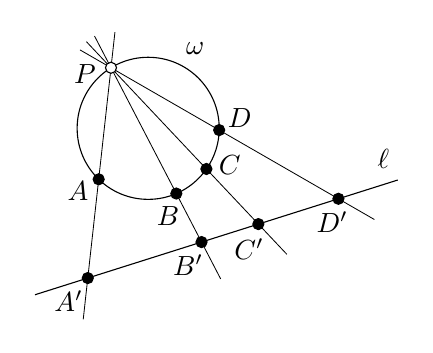
\begin{tikzpicture}[x=0.52cm,y=0.52cm]
				\clip (-0.09,-1.76) rectangle (9.13,5.5);
				\draw (2.853,3.042) circle (1.735);
				\coordinate (P) at (1.945,4.521);
				\coordinate (A) at (1.644,1.797);
				\coordinate (B) at (3.54,1.449);
				\coordinate (C) at (4.275,2.049);
				\coordinate (D) at (4.587,2.999);
				\coordinate (A1) at (1.378,-0.615);
				\coordinate (B1) at (4.156,0.264);
				\coordinate (C1) at (5.544,0.703);
				\coordinate (D1) at (7.499,1.321);
				\draw [line width=0.3,shorten <=-3ex,shorten >=-1.5em] (P) to (A1);
				\draw [line width=0.3,shorten <=-3ex,shorten >=-1.5em] (P) to (B1);
				\draw [line width=0.3,shorten <=-3ex,shorten >=-1.5em] (P) to (C1);
				\draw [line width=0.3,shorten <=-3ex,shorten >=-1.5em] (P) to (D1);
				\draw [shorten <=-2em,shorten >=-2.25em] (A1) to (D1);
				\draw [fill=white] (P) circle (2pt) node[shift={(193:2.25ex)}] {$P$};
				\draw [fill=black] (A) circle (2pt) node[shift={(210:2ex)}] {$A$};
				\draw [fill=black] (B) circle (2pt) node[shift={(250:2ex)}] {$B$};
				\draw [fill=black] (C) circle (2pt) node[shift={(10:2ex)}] {$C$};
				\draw [fill=black] (D) circle (2pt) node[shift={(30:2ex)}] {$D$};
				\draw [fill=black] (A1) circle (2pt) node[shift={(230:2.5ex)}] {$A'$};
				\draw [fill=black] (B1) circle (2pt) node[shift={(240:2.25ex)}] {$B'$};
				\draw [fill=black] (C1) circle (2pt) node[shift={(250:2.25ex)}] {$C'$};
				\draw [fill=black] (D1) circle (2pt) node[shift={(255:2ex)}] {$D'$};
				\node at (8.6,2.3) {$\ell$};
				\node at (4,5) {$\omega$};
			\end{tikzpicture} & \\
			& Fall~\ref{itm:projAbb:GG} & & Fall~\ref{itm:projAbb:GK} &
		\end{tabularx}
	\end{figure}
	\begin{figure}[ht]
		\centering
		\begin{tabularx}{\textwidth}{X c X c X}
			& 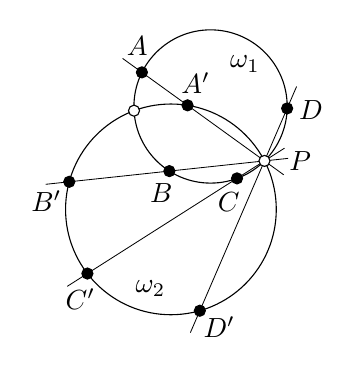
\begin{tikzpicture}[x=0.6cm,y=0.6cm]
				\clip (-1.2,-2.02) rectangle (5.12,4.62);
				\draw (2.671,2.952) circle (1.622);
				\draw (1.832,0.774) circle (2.23);
				\coordinate (P) at (3.812,1.8);
				\coordinate (A) at (1.218,3.674);
				\coordinate (B) at (1.799,1.584);
				\coordinate (C) at (3.231,1.43);
				\coordinate (D) at (4.292,2.911);
				\coordinate (A1) at (2.184,2.976);
				\coordinate (B1) at (-0.32,1.358);
				\coordinate (C1) at (0.064,-0.584);
				\coordinate (D1) at (2.444,-1.371);
				\draw [line width=0.3,shorten <=-2ex,shorten >=-2ex] (P) to (A);
				\draw [line width=0.3,shorten <=-2ex,shorten >=-2ex] (P) to (B1);
				\draw [line width=0.3,shorten <=-2ex,shorten >=-2ex] (P) to (C1);
				\draw [line width=0.3,shorten <=-2ex,shorten >=-2ex] (D) to (D1);
				\draw [fill=white] (P) circle (2pt) node[shift={(0:3ex)}] {$P$};
				\draw [fill=white] (1.051,2.863) circle (2pt);
				\draw [fill=black] (A) circle (2pt) node[shift={(100:2.25ex)}] {$A$};
				\draw [fill=black] (B) circle (2pt) node[shift={(250:2ex)}] {$B$};
				\draw [fill=black] (C) circle (2pt) node[shift={(251:2.125ex)}] {$C$};
				\draw [fill=black] (D) circle (2pt) node[shift={(-5:2ex)}] {$D$};
				\draw [fill=black] (A1) circle (2pt) node[shift={(70:2ex)}] {$A'$};
				\draw [fill=black] (B1) circle (2pt) node[shift={(220:2.5ex)}] {$B'$};
				\draw [fill=black] (C1) circle (2pt) node[shift={(255:2.25ex)}] {$C'$};
				\draw [fill=black] (D1) circle (2pt) node[shift={(320:2.125ex)}] {$D'$};
				\node at (3.4,3.85) {$\omega_1$};
				\node at (1.4,-0.90) {$\omega_2$};
			\end{tikzpicture} & & 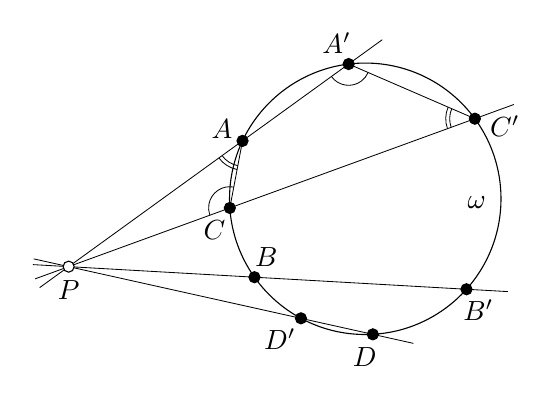
\begin{tikzpicture}[x=0.55cm,y=0.55cm]
				\clip (-3.52,-1.62) rectangle (7.93,6.29);
				\draw (4.275,2.339) circle (3.134);
				\coordinate (P) at (-2.574,0.772);
				\coordinate (A) at (1.441,3.676);
				\coordinate (B) at (1.717,0.528);
				\coordinate (C) at (1.148,2.127);
				\coordinate (D) at (4.45,-0.791);
				\coordinate (A1) at (3.891,5.45);
				\coordinate (B1) at (6.612,0.25);
				\coordinate (C1) at (6.806,4.188);
				\coordinate (D1) at (2.79,-0.421);
				\draw [line width=0.3,shorten <=-3ex,shorten >=-1.5em] (P) to (A1);
				\draw [line width=0.3,shorten <=-3ex,shorten >=-1.5em] (P) to (B1);
				\draw [line width=0.3,shorten <=-3ex,shorten >=-1.5em] (P) to (C1);
				\draw [line width=0.3,shorten <=-3ex,shorten >=-1.5em] (P) to (D);
				\draw [line width=0.3] (A) to (C);
				\draw [line width=0.3] (A1) to (C1);
				\draw [line width=0.3,shift={(A)}] (215.888:0.32cm) arc (215.888:259.306:0.32cm);
				\draw [line width=0.3,shift={(A)}] (215.888:0.37cm) arc (215.888:259.306:0.37cm);
				\draw [line width=0.3,shift={(C)}] (79.306:0.27cm) arc (79.306:200.012:0.27cm);
				\draw [line width=0.3,shift={(A1)}] (215.888:0.27cm) arc (215.888:336.594:0.27cm);
				\draw [line width=0.3,shift={(C1)}] (156.594:0.32cm) arc (156.594:200.012:0.32cm);
				\draw [line width=0.3,shift={(C1)}] (156.594:0.37cm) arc (156.594:200.012:0.37cm);
				\draw [fill=white] (P) circle (2pt) node[shift={(270:2ex)}] {$P$};
				\draw [fill=black] (A) circle (2pt) node[shift={(150:2ex)}] {$A$};
				\draw [fill=black] (B) circle (2pt) node[shift={(60:2ex)}] {$B$};
				\draw [fill=black] (C) circle (2pt) node[shift={(235:2.25ex)}] {$C$};
				\draw [fill=black] (D) circle (2pt) node[shift={(250:2ex)}] {$D$};
				\draw [fill=black] (A1) circle (2pt) node[shift={(120:2ex)}] {$A'$};
				\draw [fill=black] (B1) circle (2pt) node[shift={(300:2ex)}] {$B'$};
				\draw [fill=black] (C1) circle (2pt) node[shift={(-14:2.6ex)}] {$C'$};
				\draw [fill=black] (D1) circle (2pt) node[shift={(225:2.5ex)}] {$D'$};
				\node at (6.85,2.25) {$\omega$};
			\end{tikzpicture} & \\
			& Fall~\ref{itm:projAbb:KK} & & Fall~\ref{itm:projAbb:K} &
		\end{tabularx}
	\end{figure}
	
	Im Fall~\ref{itm:projAbb:K} müssen wir ein wenig mehr arbeiten. Mit einer einfachen Fallunterscheidung sehen wir zunächst, dass $(A,B;C,D)$ und $(A',B';C',D')$ das gleiche Vorzeichen haben. Wir müssen also nur ihre Beträge vergleichen. Dazu beobachten wir, dass die Dreiecke $PCA$ und $PA'C'$ ähnlich sind; je nachdem, ob $P$ innerhalb oder außerhalb von~$\omega$ liegt, benutzen wir dazu das Argument aus dem Beweis des Sehnen- oder des Sekantensatzes. Es folgt $\abs{A'C'}/\abs{AC}=\abs{PA'}/\abs{PC}$. Analog erhalten wir $\abs{C'B'}/\abs{CB}=\abs{PC'}/\abs{PB}$, $\abs{A'D'}/\abs{AD}=\abs{PA'}/\abs{PD}$ und $\abs{D'B'}/\abs{DB}=\abs{PD'}/\abs{PB}$. Setzen wir diese Gleichungen ein, erhalten wir
	\begin{equation*}
		\frac{\abs{(A',B';C',D')}}{\abs{(A,B;C,D)}}=\frac{\abs{PA'}}{\abs{PC}}\cdot \frac{\abs{PB}}{\abs{PC'}}\cdot \frac{\abs{PD}}{\abs{PA'}}\cdot\frac{\abs{PD'}}{\abs{PB}}=\frac{\abs{PD}\cdot\abs{PD'}}{\abs{PC}\cdot \abs{PC'}}=1\,,
	\end{equation*}
	wie gewünscht. Im letzten Schritt haben wir, je nach Lage von $P$, den Sehnensatz oder den Sekantensatz benutzt.
\end{proof}

Um die bisher ziemlich trockene Theorie auf vortreffliche Weise zu illustrieren, werden wir jetzt den Satz von Pascal auf sehr elegante Weise beweisen.

\begin{satzmitnamen}[Satz von Pascal]
	Seien $A$,~$B$, $C$, $D$, $E$ und~$F$ sechs Punkte auf einem Kreis~$\omega$. Sei $P$ der Schnittpunkt von $AB$ und~$DE$, sei $Q$ der Schnittpunkt von $BC$ und~$EF$ und schließlich sei $R$ der Schnittpunkt von $CD$ und~$FA$. Dann liegen $P$,~$Q$ und~$R$ auf einer Geraden.
\end{satzmitnamen}

\begin{figure}[ht]
	\centering
	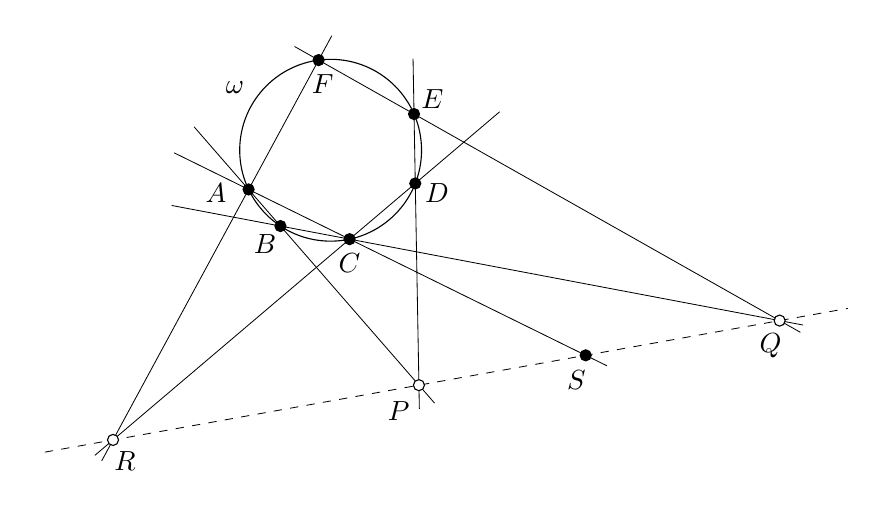
\begin{tikzpicture}[x=0.45cm,y=0.45cm]
		\clip (-3.25,-0.05) rectangle (20.25,12.7);
		\draw (5.3,9.241) circle (2.566);
		\coordinate (A) at (2.985,8.134);
		\coordinate (B) at (3.884,7.101);
		\coordinate (C) at (5.835,6.731);
		\coordinate (D) at (7.689,8.305);
		\coordinate (E) at (7.654,10.263);
		\coordinate (F) at (4.961,11.785);
		\coordinate (P) at (7.792,2.611);
		\coordinate (Q) at (17.972,4.433);
		\coordinate (R) at (-0.841,1.065);
		\coordinate (S) at (12.498,3.453);
		\draw [line width=0.3,shorten <=-3em,shorten >=-2ex] (A) to (P);
		\draw [line width=0.3,shorten <=-2em,shorten >=-2ex] (E) to (P);
		\draw [line width=0.3,shorten <=-4em,shorten >=-2ex] (B) to (Q);
		\draw [line width=0.3,shorten <=-1em,shorten >=-2ex] (F) to (Q);
		\draw [line width=0.3,shorten <=-1em,shorten >=-2ex] (F) to (R);
		\draw [line width=0.3,shorten <=-4em,shorten >=-2ex] (D) to (R);
		\draw [line width=0.3,dashed,shorten <=-2.5em,shorten >=-2.5em] (R) to (Q);
		\draw [line width=0.3,shorten <=-3em,shorten >=-2ex] (A) to (S);
		\draw [fill=black] (A) circle (2pt) node[shift={(187:2.75ex)}] {$A$};
		\draw [fill=black] (B) circle (2pt) node[shift={(230:2ex)}] {$B$};
		\draw [fill=black] (C) circle (2pt) node[shift={(270:2ex)}] {$C$};
		\draw [fill=black] (D) circle (2pt) node[shift={(335:2ex)}] {$D$};
		\draw [fill=black] (E) circle (2pt) node[shift={(40:2ex)}] {$E$};
		\draw [fill=black] (F) circle (2pt) node[shift={(280:2ex)}] {$F$};
		\draw [fill=white] (P) circle (2pt) node[shift={(232:2.75ex)}] {$P$};
		\draw [fill=white] (Q) circle (2pt) node[shift={(250:2.25ex)}] {$Q$};
		\draw [fill=white] (R) circle (2pt) node[shift={(300:2ex)}] {$R$};
		\draw [fill=black] (S) circle (2pt) node[shift={(250:2.25ex)}] {$S$};
		\node at (2.6,11) {$\omega$};
	\end{tikzpicture}
\end{figure}

\begin{proof}
	Seien $R'$~und~$R''$ die Schnittpunkte von $CD$ und~$FA$ mit~$PQ$. Wir werden $R'=R''$ und damit die Behauptung zeigen. Zu diesem Zweck betrachten wir die folgenden vier Abbildungen:
	\begin{itemize}
		\item Sei $\pi_C\colon PQ\to \omega$ die Projektion durch~$C$.
		\item Sei $\pi_P\colon \omega\to \omega$ die Projektion durch~$P$.
		\item Sei $\pi_Q\colon \omega\to \omega$ die Projektion durch~$Q$.
		\item Sei $\pi_A\colon \omega\to PQ$ die Projektion durch~$A$.
	\end{itemize}
	Wir haben gesehen, dass alle diese Abbildungen projektiv sind. Sei nun $S$ der Schnittpunkt von $AC$ und~$PQ$. Indem wir die obigen Abbildungen nacheinander anwenden, erhalten wir
	\begin{equation*}
		(P,Q;S,R')\overset{\raisebox{0.5ex}{$\scriptstyle\pi_C$}}{=}(PC\cap\omega,B;A,D)\overset{\raisebox{0.5ex}{$\scriptstyle\pi_P$}}{=}(C,A;B,E)\overset{\raisebox{0.5ex}{$\scriptstyle\pi_Q$}}{=}(B,QA\cap\omega;C,F)\overset{\raisebox{0.5ex}{$\scriptstyle\pi_A$}}{=}(P,Q;S,R'')
	\end{equation*} 
	(hierbei bezeichnet $PC\cap \omega$ den von~$C$ verschiedenen Schnittpunkt von~$PC$ mit~$\omega$ und analog bezeichnet $QA\cap \omega$ den von~$A$ verschiedenen Schnittpunkt von~$QA$ mit~$\omega$). Für jede reelle Zahl $\lambda\neq 0,1$ gibt es aber genau einen Punkt~$Y_\lambda$ auf~$PQ$, für den $(P,Q;S,Y_\lambda)=\lambda$ gilt (wir erlauben natürlich auch $Y_\lambda=\infty_{PQ}$). Also muss $R'=R''$ gelten und wir sind fertig.
\end{proof}

Mit dem gleichen Argument, mit dem wir im obigen Beweis $R'=R''$ schlussfolgern, lässt sich beweisen, dass zwei projektive Abbildungen, die in drei Punkten übereinstimmen, schon gleich sein müssen. Dieser Fakt ist sehr wichtig für die allgemeine Theorie von projektiven Abbildungen. Wir hätten den obigen Beweis auch so formulieren können, dass wir die Hintereinanderausführung $\pi_A\circ\pi_Q\circ\pi_P\circ\pi_C\colon PQ\to PQ$ betrachten und bemerken, dass diese die Punkte $P$,~$Q$ und~$S$ auf sich selbst abbildet, sodass sie mit der Identitätsabbildung $\mathrm{id}_{PQ}\colon PQ\to PQ$ übereinstimmen muss. Für Olympiadezwecke ist es aber meistens einfacher, direkt auf Doppelverhältnisjagd zu gehen. 

An dem Beweis des Satzes von Pascal ist unter anderem bemerkenswert, dass er vollkommen ohne Lagediskussion auskommt. Die Punkte $A$,~$B$, $C$, $D$, $E$ und~$F$ dürfen also in beliebiger Reihenfolge auf dem Kreis~$\omega$ liegen. Dank der projektiven Ebene müssen wir noch nicht einmal die Spezialfälle betrachten, dass einige der Geraden parallel sind, da in der projektiven Ebene auch in diesem Fall die entsprechenden Schnittpunkte definiert sind.

Außerdem lässt sich der Beweis leicht auf andere Situationen übertragen. Betrachte zum Beispiel den Fall, dass die sechs Punkte $A$,~$B$, $C$, $D$, $E$ und~$F$ nicht auf einem Kreis~$\omega$, sondern (abwechselnd) auf zwei Geraden $\ell_1$~und~$\ell_2$ liegen. Die Projektionen durch $C$,~$P$, $Q$ und~$A$ sind immer noch projektive Abbildungen $\pi_C\colon PQ\to \ell_2$, $\pi_P\colon \ell_2\to \ell_1$, $\pi_Q\colon \ell_1\to\ell_2$ und $\pi_A\colon \ell_2\to PQ$. Wir können also mit haargenau dem gleichen Argument auch den folgenden Satz zeigen:

\begin{satzmitnamen}[Satz von Pappos]
	Seien $A$,~$C$ und~$E$ drei Punkte auf einer Geraden~$\ell_1$ und $B$,~$D$ und~$F$ drei Punkte auf einer Geraden~$\ell_2$. Sei $P$ der Schnittpunkt von $AB$ und~$DE$, sei $Q$ der Schnittpunkt von $BC$ und~$EF$ und schließlich sei $R$ der Schnittpunkt von $CD$ und~$FA$. Dann liegen $P$,~$Q$ und~$R$ auf einer Geraden.
\end{satzmitnamen}

Die Sätze von Pascal und Pappos sind häufig nützlich in Olympiadeaufgaben, nicht zuletzt deshalb, weil sie nicht zum Standardrepertoire gehören und euch deshalb einen Vorteil verschaffen können.

Wir werden jetzt den Einsatz von Pascal und Pappos an zwei Beispielaufgaben demonstrieren.

\begin{aufgabe*}\label{aufgabe:InkreisPascal}
	Sei $ABC$ ein Dreieck mit Umkreis~$\Omega$. Ein Kreis~$\omega$ berühre die Strecke~$\overline{AB}$ in~$P$, die Strecke~$\overline{AC}$ in~$Q$ sowie den Umkreis~$\Omega$ von innen. Zeige, dass der Inkreismittelpunkt von $ABC$ auf der Geraden~$PQ$ liegt.
\end{aufgabe*}
\begin{figure}[ht]
	\centering
	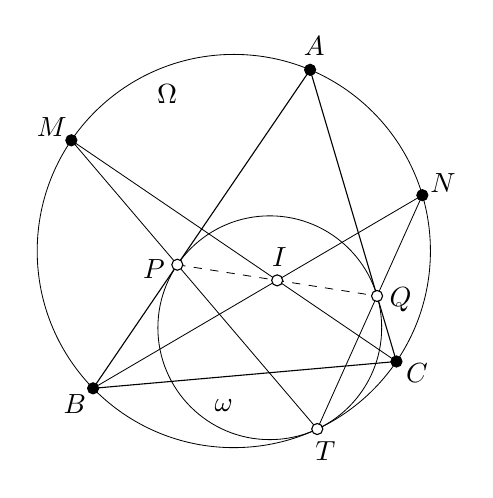
\begin{tikzpicture}[x=0.45cm,y=0.45cm]
		\draw [line width=0.3] (8.382,6.366) circle (5.549);
		\draw [line width=0.3] (9.397,4.201) circle (3.158);
		\coordinate (A) at (10.536,11.48);
		\coordinate (B) at (4.411,2.491);
		\coordinate (C) at (12.972,3.248);
		\coordinate (I) at (9.606,5.538);
		\coordinate (M) at (3.797,9.491);
		\coordinate (N) at (13.703,7.941);
		\coordinate (P) at (6.788,5.979);
		\coordinate (Q) at (12.425,5.097);
		\coordinate (T) at (10.737,1.342);
		\draw (A) to (B) to (C) to cycle;
		\draw [line width=0.3] (T) to (M) to (C);
		\draw [line width=0.3] (T) to (N) to (B);
		\draw [dashed,line width=0.3] (P) to (Q);
		\draw [fill=black] (A) circle (2pt) node[shift={(80:2ex)}] {$A$};
		\draw [fill=black] (B) circle (2pt) node[shift={(220:2ex)}] {$B$};
		\draw [fill=black] (C) circle (2pt) node[shift={(330:2ex)}] {$C$};
		\draw [fill=white] (I) circle (2pt) node[shift={(85:2ex)}] {$I$};
		\draw [fill=black] (M) circle (2pt) node[shift={(145:2ex)}] {$M$};
		\draw [fill=black] (N) circle (2pt) node[shift={(30:2ex)}] {$N$};
		\draw [fill=white] (P) circle (2pt) node[shift={(190:2ex)}] {$P$};
		\draw [fill=white] (Q) circle (2pt) node[shift={(-10:2ex)}] {$Q$};
		\draw [fill=white] (T) circle (2pt) node[shift={(290:2ex)}] {$T$};
		\node at (8.1,2) {$\omega$};
		\node at (6.5,10.8) {$\Omega$};
	\end{tikzpicture}
\end{figure}

\begin{proof}[Lösung]
	Sei $T$ der Berührpunkt der Kreise $\omega$~und~$\Omega$. Sei $M$ der von~$T$ verschiedene Schnittpunkt von~$TP$ mit~$\Omega$ und sei $N$ der von~$T$ verschiedene Schnittpunkt von~$TQ$ mit~$\Omega$. Nach dem Kreisberührungslemma ist $M$ der Mittelpunkt des Bogens~$\wideparen{AB}$ und $N$ der Mittelpunkt des Bogens~$\wideparen{CA}$. Dieses Lemma findet ihr zum Beispiel im Kapitel \emph{\embrace{Dreh-}Streckungen} im Heft für Klasse~10 (und ihr solltet es auf jeden Fall kennen); es lässt sich leicht beweisen, indem ihr die Streckung mit Zentrum~$T$ betrachtet, die $\omega$~auf~$\Omega$ abbildet. Insbesondere sind $BN$ und~$CM$ die Winkelhalbierenden von $\winkel CBA$ und $\winkel ACB$ und schneiden sich im Inkreismittelpunkt von $ABC$. Nach dem Satz von Pascal im Sehnensechseck $ABNTMC$ liegen $P$,~$Q$ und der Schnittpunkt von $BN$ und~$CM$ auf einer Geraden. Damit sind wir schon fertig.
\end{proof}


\begin{aufgabe*}[*]\label{aufgabe:VAIMO2020_2}
	Sei $ABCD$ ein Parallelogramm mit $\abs{AC}=\abs{AD}$. Sei $P$ ein Punkt auf der Verlängerung von~$\overline{AB}$ über~$B$ hinaus. Der Umkreis $\odot ACD$ und die Strecke~$\overline{PD}$ schneiden sich außer in~$D$ noch in einem Punkt~$Q$. Der Umkreis $\odot APQ$ und die Strecke~$\overline{PC}$ schneiden sich außer in~$P$ noch noch in einem Punkt~$R$. Beweise, dass sich die drei Geraden $CD$, $AQ$ und~$BR$ in einem Punkt schneiden.
\end{aufgabe*}

\begin{figure}[ht]
	\centering
	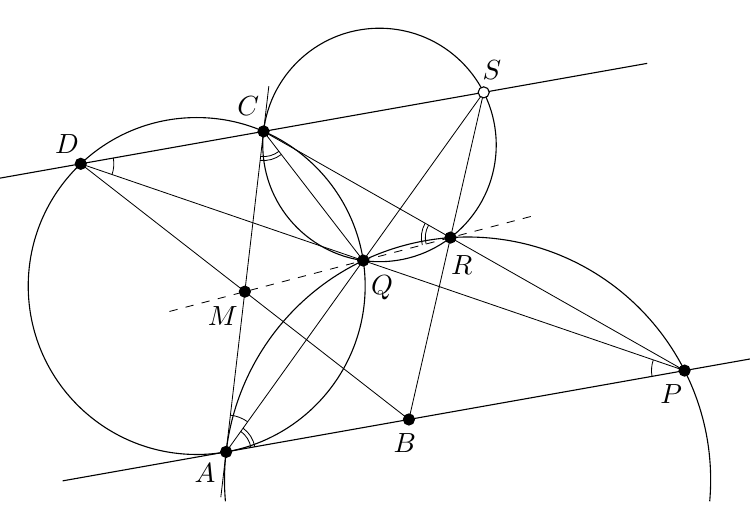
\begin{tikzpicture}[x=0.5cm,y=0.5cm]
		\draw (8.241,5.617) circle (4.279);
		\draw [shift={(15.121,0.688)}] (-5:6.174) arc (-5:185:6.174);
		\draw (12.884,9.2) circle (2.965);
		\coordinate (A) at (8.988,1.404);
		\coordinate (B) at (13.631,2.227);
		\coordinate (C) at (9.939,9.544);
		\coordinate (D) at (5.296,8.721);
		\coordinate (M) at (9.464,5.474);
		\coordinate (P) at (20.633,3.469);
		\coordinate (Q) at (12.47,6.264);
		\coordinate (R) at (14.687,6.847);
		\coordinate (S) at (15.531,10.536);
		\draw [shorten <=-6em,shorten >=-3em] (A) to (P);
		\draw [shorten <=-3em,shorten >=-6em] (D) to (S);
		\draw [line width=0.3] (A) to (S) to (B) to (D) to (P) to (C) to (Q);
		\draw [line width=0.3,shorten <=-1.65em,shorten >=-1.65em] (C) to (A); 
		\draw [line width=0.3,dashed,shorten <=-3em,shorten >=-3em] (R) to (M);
		\draw [line width=0.3, shift={(R)}] (150.398:0.32cm) arc (150.398:194.721:0.32cm);
		\draw [line width=0.3, shift={(R)}] (150.398:0.37cm) arc (150.398:194.721:0.37cm);
		\draw [line width=0.3, shift={(A)}] (10.054:0.32cm) arc (10.054:54.377:0.32cm);
		\draw [line width=0.3, shift={(A)}] (10.054:0.37cm) arc (10.054:54.377:0.37cm);
		\draw [line width=0.3, shift={(C)}] (263.335:0.32cm) arc (263.335:307.658:0.32cm);
		\draw [line width=0.3, shift={(C)}] (263.335:0.37cm) arc (263.335:307.658:0.37cm);
		\draw [line width=0.3, shift={(D)}] (-18.904:0.42cm) arc (-18.904:10.054:0.42cm);
		\draw [line width=0.3, shift={(A)}] (54.377:0.47cm) arc (54.377:83.335:0.47cm);
		\draw [line width=0.3, shift={(P)}] (161.096:0.42cm) arc (161.096:190.054:0.42cm);
		\draw [fill=black] (A) circle (2pt) node[shift={(225:2.5ex)}] {$A$};
		\draw [fill=black] (B) circle (2pt) node[shift={(260:2ex)}] {$B$};
		\draw [fill=black] (C) circle (2pt) node[shift={(121:2.5ex)}] {$C$};
		\draw [fill=black] (D) circle (2pt) node[shift={(125:2ex)}] {$D$};
		\draw [fill=black] (M) circle (2pt) node[shift={(228:2.75ex)}] {$M$};
		\draw [fill=black] (P) circle (2pt) node[shift={(240:2.25ex)}] {$P$};
		\draw [fill=black] (Q) circle (2pt) node[shift={(305:2.75ex)}] {$Q$};
		\draw [fill=black] (R) circle (2pt) node[shift={(292:2.5ex)}] {$R$};
		\draw [fill=white] (S) circle (2pt) node[shift={(70:2ex)}] {$S$};
	\end{tikzpicture}
\end{figure}

\begin{proof}[Lösung]
	Sei $S$ der Schnittpunkt von $AQ$ und~$CD$ und sei $R'$ der Schnittpunkt von $BS$ mit~$PC$. Wir müssen also $R=R'$ zeigen. Nach dem Satz von Pappos im Sechseck $ASBDPC$ liegen $Q$,~$R'$ und der Schnittpunkt von $BD$ und~$AC$ auf einer Geraden. Bei letzterem handelt es sich offenbar um den Diagonalenschnittpunkt des Parallelogramms $ABCD$, also um den Mittelpunkt von~$\overline{AC}$. Um $R=R'$ zu zeigen, müssen wir also nur zeigen, dass auch $QR$ durch den Mittelpunkt der Strecke~$\overline{AC}$ verläuft.
	
	Dazu bemerken wir, dass $QR$ die Potenzgerade der Kreise $\odot APQ$ und $\odot QRC$ ist. Wenn wir zeigen können, dass $AC$ eine Tangente an beide Kreise ist, sind wir fertig, denn die Potenzgerade verläuft bekanntlich durch den Mittelpunkt der Strecke zwischen den beiden Berührpunkten. Das ist nun eine einfache Winkeljagd: Nach dem Peripheriewinkelsatz im Sehnenviereck $AQCD$ und dem Wechselwinkelsatz gilt $\winkel QAC=\winkel QDC=\winkel QPA$. Nach der Umkehrung des Sehnen-Tangentenwinkelsatzes ist $AC$ also eine Tangente an $\odot APQ$. Im Sehnenviereck $APRQ$ gilt $\winkel CRQ=180^\circ-\winkel QRP=\winkel PAQ$. Nach Voraussetzung ist das Dreieck $ACD$ gleichschenklig mit Spitze~$A$. Also ist die Parallele zu~$CD$ durch~$A$ eine Tangente an $\odot ACD$. Nach dem Sehnen-Tangentenwinkelsatz folgt $\winkel PAQ=\winkel ACQ$. Also gilt $\winkel CRQ=\winkel ACQ$ und nach der Umkehrung des Sehnen-Tangentenwinkelsatzes folgt, dass $AC$ auch eine Tangente an $\odot QRC$ ist. Wie oben erklärt wurde, sind wir damit fertig.
\end{proof}


Es mag bisher der Eindruck entstanden sein, dass alle projektiven Abbildungen durch Projektionen gegeben sind. Das ist tatsächlich \emph{nicht} der Fall, wie ihr in der folgenden Übungsaufgabe zeigen sollt.

\begin{aufgabe*}
	Seien $A$,~$B$, $C$ und~$D$ vier Punkte auf einer Gerade oder auf einem Kreis. Wir fassen $A$,~$B$, $C$ und~$D$ als Punkte in der komplexen Ebene auf und bezeichnen mit $a$,~$b$, $c$ und~$d$ die zugehörigen komplexen Zahlen.
	\begin{enumerate}
		\item Zeige, dass das Doppelverhältnis von $A$,~$B$, $C$ und~$D$ wie folgt gegeben ist:
		\begin{equation*}
			(A,B;C,D)=\frac{a-b}{c-b}\bigg/\frac{a-d}{d-b}\,.
		\end{equation*}
		\item Sei $\iota$ die Inversion am Einheitskreis in der komplexen Ebene. Sei $z\neq 0$ eine komplexe Zahl. Zeige $\iota(z)=1/\overline{z}$.
		\item Sei $\omega$ ein Kreis oder eine Gerade und sei $\omega'$ das Bild von~$\omega$ unter~$\iota$. Zeige, dass $\iota$ eine projektive Abbildung $\iota|_{\omega}\colon \omega\to\omega'$ induziert.
	\end{enumerate}
\end{aufgabe*}

\subsection*{Harmonische Punktepaare und der Satz vom vollständigen Vierseit}
\begin{definition}
	Seien $A$,~$B$, $C$ und~$D$ vier verschiedene Punkte auf einer Gerade oder einem Kreis. Wir sagen, dass $(A,B)$ und $(C,D)$ \emph{harmonische Punktepaare} sind, wenn $(A,B;C,D)=-1$ gilt.
\end{definition}

Für zwei beliebige Punktepaare hängt das Doppelverhältnis im Allgemeinen von der Reihenfolge der Punkte innerhalb der Punktepaare ab. Für harmonische Punktepaare ist das allerdings nicht der Fall: Wenn $(A,B)$ und $(C,D)$ harmonisch sind, dann sind auch $(B,A)$ und $(C,D)$ harmonisch; es gilt $(A,B;C,D)=-1=(B,A;C,D)$.

Im Unterkapitel zu Polaren werden wir sehen, wie sich harmonische Punktepaare auf einem Kreis charakterisieren lassen. Fürs Erste betrachten wir den Fall, dass die Punkte $A$,~$B$, $C$ und~$D$ auf einer Geraden liegen. Dann gibt es für jede reelle Zahl $\lambda>0$ genau zwei Punkte auf der Geraden~$AB$, die die Strecke~$\overline{AB}$ im (ungerichteten) Verhältnis~$\lambda$ teilen: Nämlich einen Punkt~$X_\lambda$ im Inneren von~$\overline{AB}$, für den (in gerichteten Streckenlängen) $AX_{\lambda}/X_{\lambda}B=\lambda$ gilt, und einen Punkt~$X_{-\lambda}$ außerhalb von~$\overline{AB}$, für den (in gerichteten Streckenlängen) mit $AX_{-\lambda}/X_{-\lambda}B=-\lambda$ gilt. Im Fall $\lambda=1$ gilt $X_{-\lambda}=\infty_{AB}$. Somit sind die Punktepaare $(A,B)$ und $(C,D)$ genau dann harmonisch, wenn es ein $\lambda >0$ gibt, sodass $C=X_\lambda$ und $D=X_{-\lambda}$ oder $C=X_{-\lambda}$ und $D=X_\lambda$ gilt.

Harmonische Punktepaare werden dadurch interessant, dass sie häufig auf natürliche Weise in euren Skizzen auftauchen. Sei zum Beispiel $ABC$ ein Dreieck und seien $W$,~$W'$ die Schnittpunkte der Innen- bzw.\ Außenwinkelhalbierenden von $\winkel ACB$ mit~$AB$. Dann teilen $W$ und $W'$ die Strecke $\overline{AB}$ bekanntlich im Verhältnis $\abs{CA}/\abs{BC}$. Aus den obigen Überlegungen folgt also, dass $(A,B)$ und $(W,W')$ harmonische Punktepaare sind. Für ein weiteres Beispiel betrachte den Mittelpunkt~$M$ einer Strecke~$\overline{AB}$; dann sind $(A,B)$ und $(M,\infty_{AB})$ harmonische Punktepaare. Ihr werdet in den Beispielaufgaben sehen, wie sich diese triviale Beobachtung auf nicht-triviale Weise ausnutzen lässt.

Die allgemeinste Quelle von harmonischen Punktepaaren ist aber durch den folgenden Satz gegeben:
\begin{satzmitnamen}[Satz vom vollständigen Vierseit]
	Gegeben sei ein vollständiges Vierseit, das heißt vier Geraden $a$,~$b$, $c$ und~$d$, die sich in sechs paarweise verschiedenen Punkten schneiden. Sei $P$ der Schnittpunkt von $a$~und~$b$ sowie $P'$~der Schnittpunkt von $c$~und~$d$. Sei $Q$ der Schnittpunkt von $a$~und~$c$ sowie $Q'$~der Schnittpunkt von $b$~und~$d$. Sei $R$ der Schnittpunkt von $a$~und~$d$ sowie $R'$~der Schnittpunkt von $b$~und~$c$. Schließlich sei $K$ der Schnittpunkt von $QQ'$ und~$RR'$, $L$~der Schnittpunkt von $RR'$ und~$PP'$ sowie $M$~der Schnittpunkt von $PP'$ und~$QQ'$. Dann sind $(P,P')$ und $(L,M)$ harmonische Punktepaare. Ebenso sind $(Q,Q')$ und $(M,K)$ sowie $(R,R')$ und $(K,L)$ harmonische Punktepaare.
\end{satzmitnamen}

\begin{figure}[ht]
	\centering
	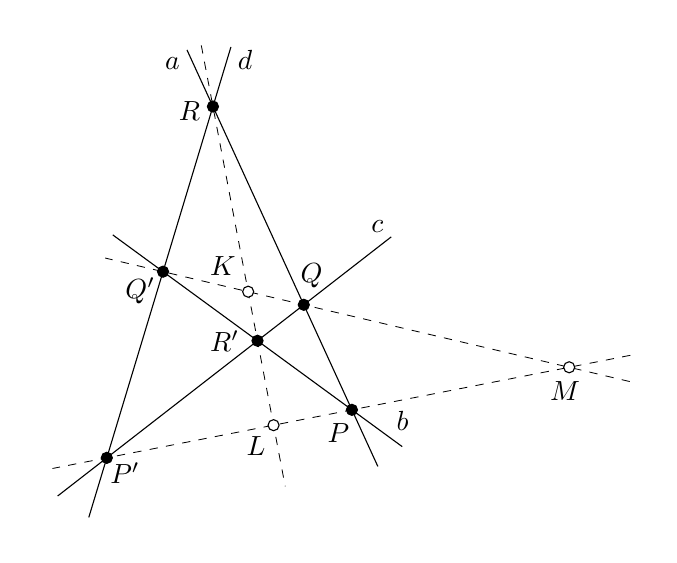
\begin{tikzpicture}[x=0.4cm,y=0.4cm]
		\clip (-5.1,-4.45) rectangle (14.62,11.65);
		\coordinate (P) at (5.195,-0.484);
		\coordinate (P1) at (-2.588,-2.008);
		\coordinate (Q) at (3.667,2.851);
		\coordinate (Q1) at (-0.802,3.903);
		\coordinate (R) at (0.782,9.146);
		\coordinate (R1) at (2.197,1.709);
		\coordinate (K) at (1.901,3.267);
		\coordinate (L) at (2.707,-0.971);
		\coordinate (M) at (12.093,0.867);
		\draw [shorten <=-2.25em,shorten >=-2.25em] (P) to (R);
		\draw [shorten <=-2.25em,shorten >=-2.25em] (P1) to (R);
		\draw [shorten <=-2.25em,shorten >=-2.25em] (P) to (Q1);
		\draw [shorten <=-2.25em,shorten >=-4em] (P1) to (Q);
		\draw [line width=0.3,dashed,shorten <=-2.25em,shorten >=-2.0em] (M) to (P1);
		\draw [line width=0.3,dashed,shorten <=-2.25em,shorten >=-2.15em] (M) to (Q1);
		\draw [line width=0.3,dashed,shorten <=-2.25em,shorten >=-2.25em] (R) to (L);
		\draw [fill=black] (P) circle (2pt) node[shift={(240:2.25ex)}] {$P$};
		\draw [fill=black] (P1) circle (2pt) node[shift={(320:2ex)}] {$P'$};
		\draw [fill=black] (Q) circle (2pt) node[shift={(75:2.5ex)}] {$Q$};
		\draw [fill=black] (Q1) circle (2pt) node[shift={(220:2.5ex)}] {$Q'$};
		\draw [fill=black] (R) circle (2pt) node[shift={(190:2ex)}] {$R$};
		\draw [fill=black] (R1) circle (2pt) node[shift={(180:2.75ex)}] {$R'$};
		\draw [fill=white] (K) circle (2pt) node[shift={(135:3ex)}] {$K$};
		\draw [fill=white] (L) circle (2pt) node[shift={(230:2.3ex)}] {$L$};
		\draw [fill=white] (M) circle (2pt) node[shift={(260:2ex)}] {$M$};
		\node at (-0.5,10.5) {$a$};
		\node at (6.8,-0.85) {$b$};
		\node at (6,5.35) {$c$};
		\node at (1.8,10.63) {$d$};
	\end{tikzpicture}
\end{figure}

\begin{proof}
	Der Satz lässt sich leicht durch eine Kombination der Sätze von Ceva und Menelaos beweisen. Mit projektiven Abbildungen ergibt sich aber eine noch kürzere Lösung. Indem wir die Gerade~$PP'$ durch~$R$ auf die Gerade~$QQ'$ projizieren, erhalten wir $(P,P';L,M)=(Q,Q';K,M)$. Indem wir die Gerade~$QQ'$ durch~$R'$ auf die Gerade~$PP'$ projizieren, erhalten wir $(Q,Q';K,M)=(P',P;L,M)$. Also ist $(P,P';L,M)=(P',P;L,M)$. Andererseits gilt ganz allgemein $(P',P;L,M)=1/(P,P';L,M)$. Also muss $(P,P';L,M)^2=1$ gelten. Da Doppelverhältnisse nie den Wert~$1$ annehmen, kommt nur $(P,P';L,M)=-1$ in Frage und es folgt, dass $(P,P')$ und $(L,M)$ in der Tat harmonisch sind. Die anderen beiden Behauptungen folgen völlig analog (oder durch geeignete Projektion).
\end{proof}

Wenn $(A,B)$ und $(C,D)$ harmonische Punktepaare sind, dann erfüllt der Mittelpunkt von $\overline{AB}$ einige sehr nützliche Relationen.

\begin{satzmitnamen}[Lemma]
	Seien $(A,B)$ und $(C,D)$ harmonische Punktepaare auf einer Geraden. Sei $M$ der Mittelpunkt der Strecke $\overline{CD}$. Dann gilt \embrace{in gerichteten Streckenlängen}
	\begin{equation*}
		AB\cdot AM=AC\cdot AD\quad\text{und}\quad AM\cdot BM=CM^2=DM^2\,.
	\end{equation*}
\end{satzmitnamen}

\begin{proof}
	Der Beweis ist eine formale Rechnung. Die Bedingung $(A,B;C,D)=-1$ impliziert $AC\cdot DB=-AD\cdot CB$. Indem wir $DB=AB-AD$ und $-CB=AC-AB$ einsetzen, erhalten wir
	\begin{equation*}
		AC\,(AB-AD)=AD\,(AC-AB)\quad\iff\quad (AC+AD)\,AB=2AC\cdot AD\,.
	\end{equation*}
	Weil $M$ der Mittelpunkt von~$\overline{CD}$ ist, gilt $AC+AD=2AM$ und die erste der beiden behaupteten Gleichheiten folgt. Andererseits gilt $AC=AM+MC$ und $AD=AM+MD=AM-MC$. Also
	\begin{equation*}
		AC\cdot AD=(AM+MC)\,(AM-MC)=AM^2-MC^2=AM^2-CM^2\,.
	\end{equation*}
	Ebenso ist $AB=AM-BM$ und somit $AB\cdot AM=(AM-BM)\,AM=AM^2-AM\cdot BM$. Indem wir die erste der beiden behaupteten Gleichheiten einsetzen, folgt die zweite.
\end{proof}

Wir werden nun harmonische Punktepaare, projektive Abbildungen, den Satz vom vollständigen Vierseit sowie das obige Lemma benutzen, um zwei Beispielaufgaben zu lösen.

\begin{aufgabe*}[*]\label{aufgabe:BWM}
	Sei $ABC$ ein nicht-gleichschenkliges Dreieck mit Inkreis $\omega$. Die Winkelhalbierende von $\winkel BAC$ schneide $BC$ in~$W$. Der Lotfußpunkt von $A$ auf $BC$ sei $L$. Schließlich sei $M$ der Mittelpunkt von~$\overline{BC}$. Die von~$BC$ verschiedene Tangente an~$\omega$ durch~$M$ berühre den Kreis~$\omega$ in~$T$. Beweise, dass $\winkel MTW=\winkel TLM$.
\end{aufgabe*}

	\begin{figure}[ht]
	\centering
	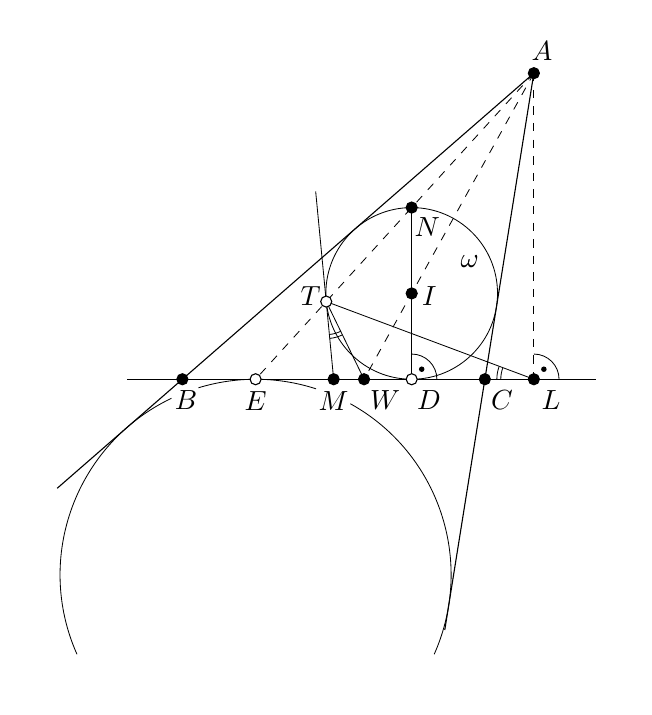
\begin{tikzpicture}[x=0.5cm,y=0.5cm]
		\clip (-3.93,-7.8) rectangle (11.21,8.93);
		\draw [line width=0.3] (5.824,2.18) coordinate (I) circle (2.18);
		\draw [line width=0.3,shift={(1.859,-4.966)}] (-24:4.966) arc (-24:61:4.966);
		\draw [line width=0.3,shift={(1.859,-4.966)}] (72:4.966) arc (72:107:4.966);
		\draw [line width=0.3,shift={(1.859,-4.966)}] (115.5:4.966) arc (115.5:204:4.966);
		\coordinate (A) at (8.927,7.774);
		\coordinate (B) at (0,0);
		\coordinate (C) at (7.683,0);
		\coordinate (D) at (5.824,0);
		\coordinate (E) at (1.859,0);
		\coordinate (L) at (8.927,0);
		\coordinate (M) at (3.842,0);
		\coordinate (N) at (5.824,4.361);
		\coordinate (T) at (3.653,1.973);
		\coordinate (W) at (4.614,0);
		\draw [shorten >=-6em] (A) to (B);
		\draw [shorten >=-9.175em] (A) to (C);
		\draw [shorten <=-2em,shorten >=-4em] (B) to (C);
		\draw [line width=0.3,dashed] (A) to (E);
		\draw [line width=0.3,dashed] (A) to (W);
		\draw [line width=0.3,dashed] (A) to (L);
		\draw [line width=0.3] (W) to (T) to (L);
		\draw [line width=0.3,shorten >=-4em] (M) to (T);
		\draw [shift={(L)},line width=0.3] (159.484:0.47cm) arc (159.484:180:0.47cm);
		\draw [shift={(L)},line width=0.3] (159.484:0.42cm) arc (159.484:180:0.42cm);
		\draw [shift={(T)},line width=0.3] (275.445:0.47cm) arc (275.445:295.961:0.47cm);
		\draw [shift={(T)},line width=0.3] (275.445:0.42cm) arc (275.445:295.961:0.42cm);
		\draw [shift={(L)},line width=0.3] (0:0.32cm) arc (0:90:0.32cm);
		\fill [shift={(L)}] (45:0.18cm) circle (1pt);
		\draw [shift={(D)},line width=0.3] (0:0.32cm) arc (0:90:0.32cm);
		\fill [shift={(D)}] (45:0.18cm) circle (1pt);
		\draw [line width=0.3] (D) to (N);
		\draw [fill=black] (A) circle (2pt) node[shift={(70:2ex)}] {$A$};
		\draw [fill=black] (B) circle (2pt) node[shift={(280:1.8ex)}] {$B$};
		\draw [fill=black] (C) circle (2pt) node[shift={(310:2.25ex)}] {$C$};
		\draw [fill=white] (D) circle (2pt) node[shift={(310:2.25ex)}] {$D$};
		\draw [fill=white] (E) circle (2pt) node[shift={(270:1.8ex)}] {$E$};
		\draw [fill=black] (I) circle (2pt) node[shift={(350:1.5ex)}] {$I$};
		\draw [fill=black] (L) circle (2pt) node[shift={(310:2.25ex)}] {$L$};
		\draw [fill=black] (M) circle (2pt) node[shift={(270:1.8ex)}] {$M$};
		\draw [fill=black] (N) circle (2pt) node[shift={(308:2.125ex)}] {$N$};
		\draw [fill=white] (T) circle (2pt) node[shift={(160:1.4ex)}] {$T$};
		\draw [fill=black] (W) circle (2pt) node[shift={(315:2.5ex)}] {$W$};
		\node at (7.3,3) {$\omega$};
	\end{tikzpicture}
\end{figure}

\begin{proof}[Lösung]
	Sei $D$ der Berührpunkt des Inkreises~$\omega$ mit~$\overline{BC}$ und sei $E$ der Berührpunkt des Ankreises gegenüber~$A$ mit~$\overline{BC}$. Schließlich sei $I$ der Inkreismittelpunkt und $N$ der Punkt auf~$\omega$, der $D$~gegenüber liegt. Bekanntlich sind $A$,~$N$ und~$E$ kollinear (wenn ihr diesen Fakt noch nicht kanntet, betrachtet die zentrische Streckung um~$A$, die den Inkreis auf den Ankreis abbildet). Außerdem ist bekannt, dass die Tangentenabschnitte am In-~und Ankreis gleich lang sind, sodass $M$ auch der Mittelpunkt von~$\overline{DE}$ ist.
	
	Nun ist $I$ der Mittelpunkt der Strecke~$\overline{DN}$, also sind $(D,N)$ und $(I,\infty_{DN})$ harmonische Punktepaare. Betrachte die Projektion $\pi_A\colon DN\to BC$ durch~$A$. Bei dieser Projektion werden offenbar $D$,~$I$ und~$N$ auf $D$,~$W$ und~$E$ abgebildet. Außerdem ist $A\infty_{DN}$ die Parallele zu~$DN$ durch~$A$. Weil $DN$ senkrecht auf~$BC$ steht, muss $A\infty_{DN}$ das Lot von~$A$ auf~$BC$ sein und es folgt $\pi_A(\infty_{DN})=L$. Also sind $(D,E)$ und $(W,L)$ harmonische Punktepaare. Weil $M$ der Mittelpunkt von $\overline{DE}$ ist, zeigt das Lemma $WM\cdot LM=DM^2$. Weil die Tangentenabschnitte $\overline{DM}$ und~$\overline{TM}$ gleich lang sind, gilt außerdem $DM^2=TM^2$. Indem wir zu ungerichteten Streckenlängen übergehen, folgt $\abs{MW}\cdot\abs{ML}=\abs{MT}^2$ und nach Umstellen $\abs{MW}/\abs{MT}=\abs{MT}/\abs{ML}$. Die Dreiecke $MWT$ und $MLT$ haben den Winkel $\winkel WMT=\winkel LMT$ gemeinsam und stimmen im Verhältnis der anliegenden Seiten überein. Also sind sie ähnlich und es folgt wie gewünscht $\winkel MTW=\winkel TLM$.
\end{proof}

Die Skizze legt außerdem nahe, dass $T$ auf der Geraden durch $A$,~$N$ und~$E$ liegt. Das ist in der Tat der Fall und ihr sollt es in Übungsaufgabe~\ref{aufgabe:BWM2} zeigen.

\begin{aufgabe*}[*]\label{aufgabe:VAIMO2008_5}
	Sei $ABCD$ ein konvexes Sehnenviereck. Die Diagonalen $AC$ und~$BD$ schneiden sich in~$E$ und die Geraden $AD$ und~$BC$ schneiden sich in~$F$. Seien $M$~und~$N$ die Mittelpunkte der Seiten $\overline{AB}$ und~$\overline{CD}$. Zeige, dass die Gerade~$EF$ den Umkreis $\odot ENM$ berührt.
\end{aufgabe*}

Aufgabe~\ref{aufgabe:VAIMO2008_5} wird wesentlich machbarer, wenn ihr den folgenden Satz kennt.

\begin{satzmitnamen}[Satz von der Gauß-Newton Geraden]
	Gegeben sei ein vollständiges Vierseit, das von den Geraden $a$,~$b$, $c$ und~$d$ sowie ihren Schnittpunkten $P$,~$Q$,~$R$ und $P'$,~$Q'$,~$R'$ gebildet wird \embrace{wobei die Bezeichnungen wie im Satz vom vollständigen Vierseit gewählt werden}. Seien $L$,~$M$ und~$N$ die Mittelpunkte der Diagonalen $\overline{PP'}$, $\overline{QQ'}$ und~$\overline{RR'}$. Dann sind $L$,~$M$ und~$N$ kollinear.
\end{satzmitnamen}

\begin{figure}[ht]
	\centering
	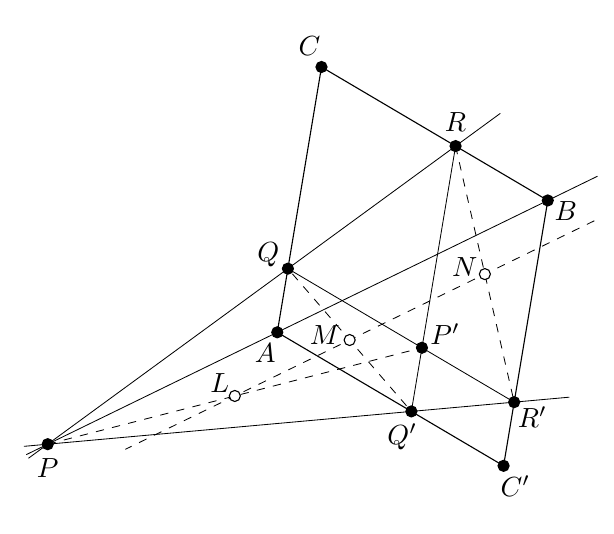
\begin{tikzpicture}[x=0.5cm,y=0.5cm]
		%\clip (-4.8,-4.15) rectangle (14.32,11.35);
		\coordinate (A) at (2.45,2.301);
		\coordinate (B) at (9.321,5.65);
		\coordinate (C) at (3.573,9.04);
		\coordinate (C1) at (8.198,-1.09);
		\coordinate (P) at (-3.381,-0.541);
		\coordinate (P1) at (6.125,1.909);
		\coordinate (Q) at (2.72,3.918);
		\coordinate (Q1) at (5.856,0.292);
		\coordinate (R) at (6.979,7.031);
		\coordinate (R1) at (8.467,0.527);
		\coordinate (L) at (1.372,0.684);
		\coordinate (M) at (4.288,2.105);
		\coordinate (N) at (7.723,3.779);
		\draw [line width=0.3,shorten <=-2ex,shorten >=-2em] (P) to (R);
		\draw [line width=0.3,shorten <=-2ex,shorten >=-2em] (P) to (R1);
		\draw [line width=0.3,shorten <=-2ex,shorten >=-2em] (P) to (B);
		\draw (A) to (C1) to (B) to (C) to cycle; 
		\draw [line width=0.3] (Q1) to (R);
		\draw [line width=0.3] (Q) to (R1);
		\draw [line width=0.3,dashed] (P) to (P1);
		\draw [line width=0.3,dashed,dash phase=3.5] (Q) to (Q1);
		\draw [line width=0.3,dashed] (R) to (R1);
		\draw [line width=0.3,dashed,shorten <=-4.4em,shorten >=-4.4em] (N) to (L);
		\draw [fill=black] (A) circle (2pt) node[shift={(240:2ex)}] {$A$};
		\draw [fill=black] (B) circle (2pt) node[shift={(-30:1.75ex)}] {$B$};
		\draw [fill=black] (C) circle (2pt) node[shift={(120:2ex)}] {$C$};
		\draw [fill=black] (C1) circle (2pt) node[shift={(300:2ex)}] {$C'$};
		\draw [fill=black] (P) circle (2pt) node[shift={(270:2ex)}] {$P$};
		\draw [fill=black] (P1) circle (2pt) node[shift={(30:2.25ex)}] {$P'$};
		\draw [fill=black] (Q) circle (2pt) node[shift={(145:2ex)}] {$Q$};
		\draw [fill=black] (Q1) circle (2pt) node[shift={(250:2.25ex)}] {$Q'$};
		\draw [fill=black] (R) circle (2pt) node[shift={(90:2ex)}] {$R$};
		\draw [fill=black] (R1) circle (2pt) node[shift={(320:2ex)}] {$R'$};
		\draw [fill=white] (L) circle (2pt) node[shift={(140:1.65ex)}] {$L$};
		\draw [fill=white] (M) circle (2pt) node[shift={(168:2.125ex)}] {$M$};
		\draw [fill=white] (N) circle (2pt) node[shift={(160:1.8ex)}] {$N$};
	\end{tikzpicture}
\end{figure}
\begin{proof}
	Betrachte die Streckung mit Zentrum~$P'$ und Faktor~$2$. Diese Streckung bildet den Mittelpunkt~$L$ von~$\overline{PP'}$ auf~$P$ ab. Der Mittelpunkt~$M$ von~$\overline{QQ'}$ wird auf denjenigen Punkt~$A$ abgebildet, für den $AQ'P'Q$ ein Parallelogramm ist und der Mittelpunkt~$N$ von~$\overline{RR'}$ wird auf denjenigen Punkt~$B$ abgebildet, für den $P'R'BR$ ein Parallelogramm ist.
	% Tien: Vielleicht willst du noch als Begründung hinschreiben, dass a priori bekannt ist das P auf QR und Q'R' liegt.
	Es genügt also, zu zeigen, dass $P$,~$A$ und~$B$ kollinear sind. Dazu sei $P_1$ der Schnittpunkt von~$QR$ mit~$AB$ und $P_2$~der Schnittpunkt von~$Q'R'$ mit~$AB$. Wir müssen dann $P_1=P_2$ zeigen.
	
	Zu diesem Zweck betrachte den Schnittpunkt~$C$ von $AQ$ und~$BR$ sowie den Schnittpunkt~$C'$ von $AQ'$ und~$BR'$. Nach dem Satz von Menelaos in den Dreiecken $ABC$ und $AC'B$ gilt
	\begin{equation*}
		\frac{AP_1}{P_1B}=-\frac{QA}{CQ}\cdot \frac{RC}{BR}\quad \text{und}\quad \frac{AP_2}{P_2B}=-\frac{Q'A}{C'Q'}\cdot \frac{R'C'}{BR'}\,.
	\end{equation*}
	Nach Konstruktion gilt aber $AC\parallel Q'R\parallel C'B$ und $AC'\parallel QR'\parallel CB$. Insbesondere ist $AC'R'Q$ ein Parallelogramm und es gilt $QA=R'C'$. Analog gilt $CQ=BR'$, $RC=Q'A$ und $BR=C'Q'$. Indem wir dies in die obigen Gleichungen einsetzen, folgt $AP_1/P_1B=AP_2/P_2B$. Für jede reelle Zahl $\lambda\neq 0$ gibt es aber genau einen Punkt~$X_\lambda$ auf~$AB$, für den (in gerichteten Streckenlängen) $AX_\lambda/X_\lambda B=\lambda$ gilt. Also muss $P_1=P_2$ gelten und wir sind fertig.
\end{proof}
\begin{figure}[ht]
	\centering
	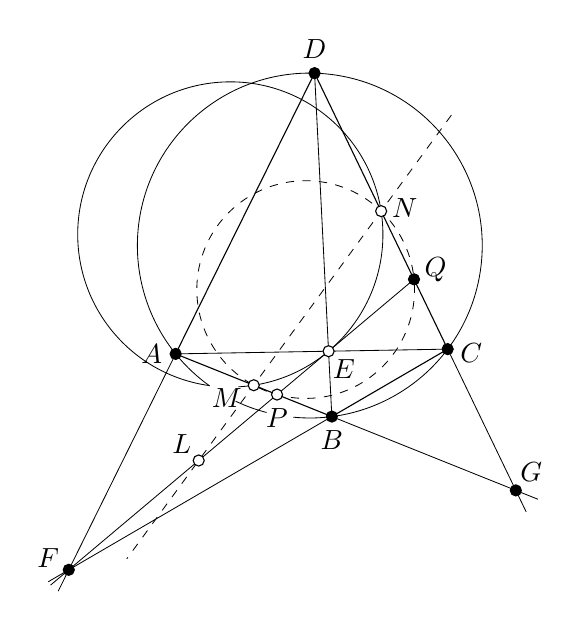
\begin{tikzpicture}[x=0.5cm,y=0.5cm]
		\clip (-1.65,-3.4) rectangle (11.65,11.15);
		\draw [line width=0.3,shift={(5.516,5.616)}] (-95.5:4.38) arc (-95.5:234.5:4.38);
		\draw [line width=0.3,shift={(5.516,5.616)}] (244.5:4.38) arc (244.5:255.5:4.38);
		\draw [line width=0.3,shift={(3.497,5.898)}] (-87:3.876) arc (-87:262:3.876);
		\draw [line width=0.3,dashed] (5.411,4.498) circle (2.765);
		\coordinate (A) at (2.108,2.864);
		\coordinate (B) at (6.076,1.272);
		\coordinate (C) at (9.018,2.985);
		\coordinate (D) at (5.637,9.995);
		\coordinate (E) at (5.993,2.932);
		\coordinate (F) at (-0.606,-2.62);
		\coordinate (G) at (10.749,-0.603);
		\coordinate (L) at (2.694,0.156);
		\coordinate (M) at (4.092,2.068);
		\coordinate (N) at (7.328,6.49);
		\coordinate (P) at (4.684,1.831);
		\coordinate (Q) at (8.163,4.758);
		\draw (A) to (B) to (C) to (D) to cycle;
		\draw [line width=0.3] (A) to (C);
		\draw [line width=0.3] (B) to (D);
		\draw [line width=0.3,shorten >=-2ex] (A) to (F);
		\draw [line width=0.3,shorten >=-2ex] (B) to (F);
		\draw [line width=0.3,shorten >=-2ex] (B) to (G);
		\draw [line width=0.3,shorten >=-2ex] (C) to (G);
		\draw [line width=0.3,shorten >=-2ex] (Q) to (F);
		\draw [dashed,line width=0.3,shorten >=-4.4em,shorten <=-4.3em] (N) to (L);
		\draw [fill=black] (A) circle (2pt) node[shift={(180:2ex)}] {$A$};
		\draw [fill=black] (B) circle (2pt) node[shift={(270:2ex)}] {$B$};
		\draw [fill=black] (C) circle (2pt) node[shift={(350:2ex)}] {$C$};
		\draw [fill=black] (D) circle (2pt) node[shift={(90:2ex)}] {$D$};
		\draw [fill=white] (E) circle (2pt) node[shift={(310:2ex)}] {$E$};
		\draw [fill=black] (F) circle (2pt) node[shift={(150:2ex)}] {$F$};
		\draw [fill=black] (G) circle (2pt) node[shift={(50:2ex)}] {$G$};
		\draw [fill=white] (L) circle (2pt) node[shift={(135:2ex)}] {$L$};
		\draw [fill=white] (M) circle (2pt) node[shift={(205:2.5ex)}] {$M$};
		\draw [fill=white] (N) circle (2pt) node[shift={(8:2ex)}] {$N$};
		\draw [fill=white] (P) circle (2pt) node[shift={(270:2ex)}] {$P$};
		\draw [fill=black] (Q) circle (2pt) node[shift={(25:2ex)}] {$Q$};
	\end{tikzpicture}
\end{figure}
\begin{proof}[Lösung zu Aufgabe~\ref{aufgabe:VAIMO2008_5}]
	Betrachte außerdem den Schnittpunkt~$G$ von $AB$ und~$CD$ sowie die Schnittpunkte $P$~und~$Q$ von~$EF$ mit $AB$ und~$CD$. Nach dem Satz vom vollständigen Vierseit (angewendet auf das Vierseit, das von $CF$, $DF$, $AC$ und $BD$ gebildet wird)
	% Tien: Vielleicht willst du noch schreiben, dass du das Vierseit FC, FD, AC, BD betrachtest.
	sind $(A,B)$ und $(P,G)$ sowie $(C,D)$ und $(Q,G)$ harmonische Punktepaare. Nach dem Lemma gilt $GP\cdot GM=GA\cdot GB$ und $GQ\cdot GN=GC\cdot GD$. Nach dem Sekantensatz gilt aber auch $GA\cdot GB=GC\cdot GD$. Also ist $GP\cdot GM=GQ\cdot GN$ und nach der Umkehrung des Sekantensatzes folgt, dass $PQNM$ ein Sehnenviereck ist.
	
	Sei nun $L$ der Mittelpunkt von $\overline{EF}$. Nach dem Satz von der Gauß-Newton-Geraden liegt $L$ auf der Geraden $MN$. Nach dem Satz vom vollständigen Vierseit (im gleichen Vierseit wie vorhin) sind $(E,F)$ und $(P,Q)$ harmonische Punktepaare. Nach dem Lemma über harmonische Punktepaare gilt somit $PL\cdot QL=EL^2$. Nach dem Sekantensatz ist $ML\cdot NL=PL\cdot QL$. Also folgt $EL^2=ML\cdot NL$ und die Umkehrung des Sekanten-Tangentensatzes liefert uns, dass $EF$ in der Tat eine Tangente an $\odot ENM$ ist. Damit sind wir fertig.
\end{proof}
Eine etwas einfachere Aufgabe, in der ähnliche Methoden zum Einsatz kommen, ist die folgende Übungsaufgabe.
\begin{aufgabe*}
	Sei $ABC$ ein Dreieck. Ein Kreis $\omega$ verläuft durch $B$ und $C$ und schneidet $AB$ in $Y$ sowie $AC$ in $Z$. Sei $P$ der Schnittpunkt von $BZ$ und $CY$ und sei $X$ der Schnittpunkt von $AP$ mit $BC$. Beweise, dass der Mittelpunkt der Strecke $\overline{BC}$ auf dem Umkreis $\odot XYZ$ liegt.
\end{aufgabe*}


\subsection*{Polaren}
%In diesem Kapitel lernt ihr eine Konstruktion kennen, mit der sich die das Dualitätsprinzip auf konkrete Weise verwirklichen lässt.
\begin{definition}
	Sei $\omega$ ein Kreis mit Mittelpunkt~$O$ und Radius~$r$. Sei $P$ ein von~$O$ verschiedener Punkt und sei $P'$ das Bild von~$P$ unter Inversion an~$\omega$, also derjenige Punkt auf dem Strahl~$\overrightarrow{OP}$, für den $\abs{OP}\cdot \abs{OP'}=r^2$ gilt. Sei $p$ die Senkrechte auf~$OP$ in~$P'$. Dann wird $p$ die \emph{Polare von~$P$} genannt. Umgekehrt nennen wir $P$ den \emph{Pol von~$p$}.
	
	Polaren lassen sich auch für Fernpunkte definieren. Wenn $\infty_\ell$ der Fernpunkt auf der Geraden~$\ell$ ist, dann definieren wir die \emph{Polare von~$\infty_\ell$} als die Senkrechte~$p$ auf~$\ell$ durch~$O$. Wenn umgekehrt $p$ eine Gerade durch~$O$ ist, definieren wir den \emph{Pol von~$p$} als~$\infty_\ell$, wobei $\ell$ die Senkrechte auf~$p$ in~$O$ ist. Die Polare von~$O$ ist schließlich die Ferngerade und umgekehrt ist $O$ der Pol der Ferngeraden. 
\end{definition}

Der wichtigste Fakt über Pole und Polaren ist der folgende:
\begin{satzmitnamen}[Satz von La~Hire, Pol-Polare-Dualität]
	Ein Punkt~$P$ liegt auf der Polaren eines weiteren Punktes~$Q$ genau dann, wenn $Q$ auf der Polaren von~$P$ liegt.
\end{satzmitnamen}

\begin{figure}[ht]
	\centering
	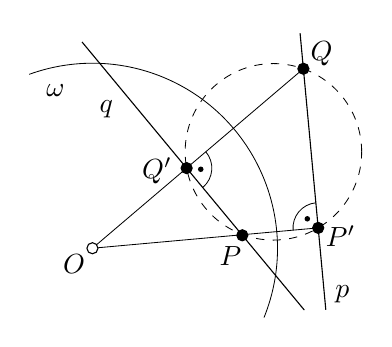
\begin{tikzpicture}[x=2.35cm,y=2.35cm]
		\clip (-0.35,-0.382) rectangle (1.464,1.192);
		\draw[line width=0.3] (-22:1) arc (-22:110:1);
		\coordinate (O) at (0,0);
		\draw[line width=0.3,dashed] (0.978,0.521) circle (0.477);
		\coordinate (P1) at (1.22,0.11);
		\coordinate (P) at (0.81,0.07);
		\coordinate (Q) at (1.14,0.97);
		\coordinate (Q1) at (0.509,0.433);
		\draw [line width=0.3] (P1) to (O) to (Q);
		\draw[shorten <=-3ex,shorten >=-6.9ex] (Q) to (P1);
		\draw[shorten <=-13.75ex,shorten >=-8.15ex] (Q1) to (P);
		\draw[line width=0.3, shift={(P1)}] (95.1:0.32cm) arc (95.1:185.1:0.32cm);
		\fill[shift={(P1)}] (140.1:0.18cm) circle (1pt);
		\draw[line width=0.3, shift={(Q1)}] (310.29:0.32cm) arc (310.29:400.29:0.32cm);
		\fill[shift={(Q1)}] (355.29:0.18cm) circle (1pt);
		\draw[fill=white] (O) circle (2pt) node[shift={(220:2ex)}] {$O$};
		\draw[fill=black] (P) circle (2pt) node[shift={(240:2ex)}] {$P$};
		\draw[fill=black] (P1) circle (2pt) node[shift={(-20:2ex)}] {$P'$};
		\draw[fill=black] (Q) circle (2pt) node[shift={(40:2ex)}] {$Q$};
		\draw[fill=black] (Q1) circle (2pt) node[shift={(185:2.5ex)}] {$Q'$};
		\node at (-0.2,0.85) {$\omega$};
		\node at (0.075,0.75) {$q$};
		\node at (1.35,-0.25) {$p$};
	\end{tikzpicture}
\end{figure}

\begin{proof}
	Seien $P'$~und~$Q'$ die Bilder von $P$~und~$Q$ unter Inversion an~$\omega$. Angenommen, $Q$~liegt auf der Polaren von~$P$, also der Senkrechten auf~$OP$ in~$P'$. Nach Konstruktion gilt $\abs{OP}\cdot \abs{OP'}=r^2=\abs{OQ}\cdot \abs{OQ'}$. Nach der Umkehrung des Sekantensatzes muss $PP'QQ'$ ein Sehnenviereck sein. Mit $\winkel QP'P=90^\circ$ folgt also auch $\winkel PQ'Q=90^\circ$. Also liegt $P$ auf der Senkrechten auf~$OQ$ in~$Q'$, sprich der Polaren von~$Q$. Die andere Implikation lässt sich völlig analog beweisen.
\end{proof}

Mithilfe des Satzes von La~Hire lassen sich Pole und Polaren bestimmen (auch wenn das erstmal ziemlich verwirrend ist).
% Tien: Die Aussage in Klammern ist nicht vollständig. Hier fehlt wohl etwas.
% Tien: Ich habe den folgenden Abschnitt etwas (meiner Meinung nach klarer) umformuliert.
Wenn zum Beispiel $P$ der Schnittpunkt zweier Geraden $a$~und~$b$ mit den Polen $A$~und~$B$ ist, dann impliziert der Satz von La~Hire, dass $AB$ die Polare von~$P$ sein muss. Für einen gegebenen Punkt~$P$, der außerhalb von~$\omega$ liegt, können wir $A$~und~$B$ als die Berührpunkte der Tangenten an~$\omega$ durch~$P$ wählen. Weil $A$~und~$B$ auf~$\omega$ liegen, werden sie durch Inversion an~$\omega$ auf sich selbst abgebildet. Folglich sind die Polaren von $A$~und~$B$ die Tangenten an~$\omega$ in $A$~und~$B$. Ihr Schnittpunkt~$P$ muss also der Pol von~$AB$ sein und umgekehrt muss $AB$ die Polare von~$P$ sein.

\begin{figure}[ht]
	\centering
	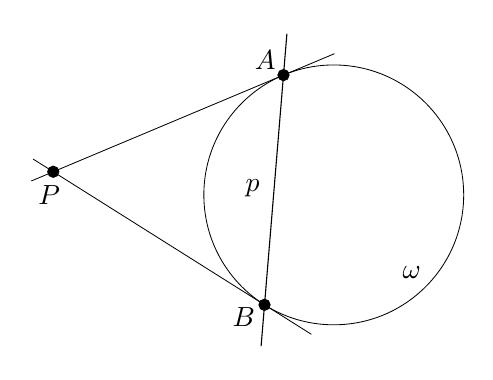
\begin{tikzpicture}[x=1.65cm,y=1.65cm]
		\clip (-2.356,-1.209) rectangle (1.012,1.287);
		%\draw[line width=0.3] (-22:1) arc (-22:110:1);
		\draw [line width=0.3] (0,0) circle (1);
		\coordinate (A) at (-0.387,0.922);
		\coordinate (B) at (-0.533,-0.846);
		\coordinate (P) at (-2.159,0.178);
		\draw [line width=0.3,shorten <=-2ex,shorten >=-2em] (P) to (A);
		\draw [line width=0.3,shorten <=-2ex,shorten >=-2em] (P) to (B);
		\draw[shorten <=-1.5em,shorten >=-1.5em] (A) to (B);
		\draw[fill=black] (P) circle (2pt) node[shift={(260:2ex)}] {$P$};
		\draw[fill=black] (A) circle (2pt) node[shift={(140:2ex)}] {$A$};
		\draw[fill=black] (B) circle (2pt) node[shift={(210:2ex)}] {$B$};
		\node at (0.6,-0.6) {$\omega$};
		\node at (-0.625,0.05) {$p$};
	\end{tikzpicture}
\end{figure}

Der Satz von La~Hire lässt sich verwenden, um Aufgaben umzuformulieren (wie immer in der Hoffnung, dass die neue Aufgabe einfacher ist). Wenn in einer Aufgabe zum Beispiel zu zeigen ist, dass sich drei Geraden in einem Punkt schneidet, könnt ihr stattdessen die Pole der Geraden bezüglich eines geeigneten Kreises betrachten und beweisen, dass die drei Pole auf einer Geraden liegen. Ein perfektes Beispiel hierfür ist die folgende Aufgabe, die ohne diesen Trick wesentlich schwieriger wäre.

\begin{aufgabe*}[*]
	Sei $ABC$ ein Dreieck mit Inkreis~$\omega$ und Inkreismittelpunkt~$I$. Sei $t$ eine Tangente an~$\omega$, die nicht durch $A$,~$B$ oder~$C$ verläuft. Wähle Punkte $A'$,~$B'$ und~$C'$ auf~$t$, sodass $\winkel AIA'=90^\circ$, $\winkel BIB'=90^\circ$ und $\winkel CIC'=90^\circ$. Beweise, dass sich die Geraden $AA'$, $BB'$ und~$CC'$ in einem Punkt schneiden.
\end{aufgabe*}

\begin{figure}[ht]
	\centering
	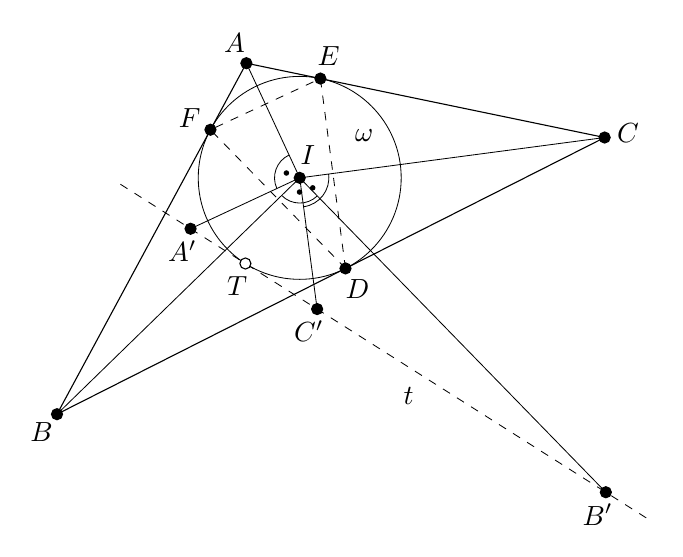
\begin{tikzpicture}[x=1.25cm,y=1.25cm]
		\clip (-2.97,-1.705) rectangle (3.403,3.391);
		%\draw[line width=0.3] (-22:1) arc (-22:110:1);
		\draw [line width=0.3] (-0.206,1.865) coordinate (I) circle (1.031);
		\coordinate (A) at (-0.748,3.03);
		\coordinate (A1) at (-1.315,1.348);
		\coordinate (B) at (-2.672,-0.536);
		\coordinate (B1) at (2.904,-1.329);
		\coordinate (C) at (2.892,2.275);
		\coordinate (C1) at (-0.029,0.532);
		\coordinate (D) at (0.259,0.945);
		\coordinate (E) at (0.004,2.874);
		\coordinate (F) at (-1.113,2.354);
		\coordinate (T) at (-0.758,0.995);
		\draw (A) to (B) to (C) to cycle;
		\draw [line width=0.3,shorten <=-3em,shorten >=-2em,dashed] (A1) to (B1);
		\draw[line width=0.3] (A) to (I) to (A1);
		\draw[line width=0.3] (B) to (I) to (B1);
		\draw[line width=0.3] (C) to (I) to (C1);
		\draw [dashed,line width=0.3] (D) to (E) to (F) to cycle;
		\draw [shift={(I)},line width=0.3] (114.972:0.32cm) arc (114.972:204.972:0.32cm);
		\fill [shift={(I)}] (159.972:0.18cm) circle (1pt);
		\draw [shift={(I)},line width=0.3] (277.548:0.37cm) arc (277.548:367.548:0.37cm);
		\fill [shift={(I)}] (322.548:0.208cm) circle (1pt);
		\draw [shift={(I)},line width=0.3] (224.233:0.32cm) arc (224.233:314.233:0.32cm);
		\fill [shift={(I)}] (269.233:0.18cm) circle (1pt);
		\draw[fill=black] (A) circle (2pt) node[shift={(120:2ex)}] {$A$};
		\draw[fill=black] (B) circle (2pt) node[shift={(230:2ex)}] {$B$};
		\draw[fill=black] (C) circle (2pt) node[shift={(10:2ex)}] {$C$};
		\draw[fill=black] (D) circle (2pt) node[shift={(300:2ex)}] {$D$};
		\draw[fill=black] (E) circle (2pt) node[shift={(70:2ex)}] {$E$};
		\draw[fill=black] (F) circle (2pt) node[shift={(150:2ex)}] {$F$};
		\draw[fill=black] (I) circle (2pt) node[shift={(70:2ex)}] {$I$};
		\draw[fill=white] (T) circle (2pt) node[shift={(250:2ex)}] {$T$};
		\draw[fill=black] (A1) circle (2pt) node[shift={(250:2ex)}] {$A'$};
		\draw[fill=black] (B1) circle (2pt) node[shift={(250:2ex)}] {$B'$};
		\draw[fill=black] (C1) circle (2pt) node[shift={(250:2ex)}] {$C'$};
		\node at (0.45,2.3) {$\omega$};
		\node at (0.9,-0.35) {$t$};
	\end{tikzpicture}
\end{figure}

\begin{proof}[Lösung]
	Wir wollen stattdessen zeigen, dass die Pole von $AA'$, $BB'$ und~$CC'$ bezüglich~$\omega$ auf einer Geraden liegen. Was ist also der Pol~$X$ von~$AA'$ bezüglich~$\omega$? Nach dem Satz von La~Hire muss $X$ der Schnittpunkt der Polaren von~$A$ und der Polaren von~$A'$ sein. Wie wir weiter oben gesehen haben, können wir die Polare von~$A$ direkt als die Gerade~$EF$ identifizieren, wobei $E$~und~$F$ die Berührpunkte des Inkreises~$\omega$ mit den Seiten $\overline{CA}$ und~$\overline{AB}$ sind. Wir müssen also nur die Polare von~$A'$ identifizieren. Sei $T$ der Berührpunkt von~$t$ an~$\omega$. Weil $A'$ auf~$t$ liegt, also auf der Polaren von~$T$, muss $T$ auf der Polaren von~$A'$ liegen. Andererseits steht die Polare von~$A'$ senkrecht auf~$A'I$. Die Polare von~$A'$ ist also die Senkrechte von~$T$ auf~$A'I$. Nach Voraussetzung ist $A'I\perp AI$. Andererseits ist aber auch $EF\perp AI$. Die Senkrechte von~$T$ auf~$A'I$ ist also auch die Senkrechte von~$T$ auf~$EF$. Insgesamt folgt, dass der Pol von~$AA'$, also der Schnittpunkt der Polaren von $A$~und~$A'$, durch den Lotfußpunkt von~$T$ auf~$EF$ gegeben ist. Analog sind die Pole von $BB'$ und~$CC'$ die Lotfußpunkte von~$T$ auf $FD$ und~$DE$, wobei $D$ der Berührpunkt von~$\omega$ mit~$\overline{BC}$ ist. Wir müssen somit zeigen, dass diese drei Lotfußpunkte kollinear sind. Das ist aber genau der Satz von der Simson-Geraden, angewendet auf das Dreieck $DEF$ und den Punkt~$T$ auf seinem Umkreis.
\end{proof}

Harmonische Punktepaare auf Kreisen lassen sich sehr elegant durch Polaren charakterisieren.

\begin{satzmitnamen}[Lemma]
	Seien $A$,~$B$, $C$ und~$D$ vier verschiedene Punkte auf einem Kreis~$\omega$. Die Punktepaare $(A,B)$ und $(C,D)$ sind genau dann harmonisch, wenn der Pol~\(P\) von~$AB$ auf~$CD$ liegt. In diesem Fall sind auch die Punktepaare $(P,Q)$ und $(C,D)$ harmonisch, wobei $Q$ den Schnittpunkt von $AB$ und~$CD$ bezeichnet.
\end{satzmitnamen}

\begin{figure}[ht]
	\centering
	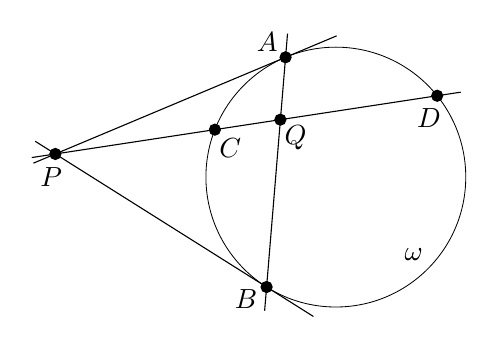
\begin{tikzpicture}[x=1.65cm,y=1.65cm]
		\clip (-2.372,-1.11) rectangle (1.012,1.15);
		%\draw[line width=0.3] (-22:1) arc (-22:110:1);
		\draw [line width=0.3] (0,0) circle (1);
		\coordinate (A) at (-0.387,0.922);
		\coordinate (B) at (-0.533,-0.846);
		\coordinate (C) at (-0.931,0.365);
		\coordinate (D) at (0.78,0.626);
		\coordinate (P) at (-2.159,0.178);
		\coordinate (Q) at (-0.427,0.442);
		\draw [shorten <=-2ex,shorten >=-2em] (P) to (A);
		\draw [shorten <=-2ex,shorten >=-2em] (P) to (B);
		\draw[shorten <=-2ex,shorten >=-2ex] (A) to (B);
		\draw [shorten <=-2ex,shorten >=-2ex] (P) to (D);
		\draw[fill=black] (P) circle (2pt) node[shift={(260:2ex)}] {$P$};
		\draw[fill=black] (Q) circle (2pt) node[shift={(310:2ex)}] {$Q$};
		\draw[fill=black] (A) circle (2pt) node[shift={(140:2ex)}] {$A$};
		\draw[fill=black] (B) circle (2pt) node[shift={(210:2ex)}] {$B$};
		\draw[fill=black] (C) circle (2pt) node[shift={(310:2ex)}] {$C$};
		\draw[fill=black] (D) circle (2pt) node[shift={(250:2ex)}] {$D$};
		\node at (0.6,-0.6) {$\omega$};
	\end{tikzpicture}
\end{figure}

\begin{proof}
	Der Pol von~$AB$ ist der Schnittpunkt der Tangenten an~$\omega$ in $A$~und~$B$. Sei $D'$ der von~$C$ verschiedene Schnittpunkt von~$PC$ mit~$\omega$. Wie wir in einem vorherigen Lemma gezeigt haben, ist die Projektion $\pi_P\colon \omega\to \omega$ durch~$P$ eine projektive Abbildung. Offenbar bildet $\pi_P$ die Punkte $A$~und~$B$ auf sich selbst ab und vertauscht $C$~und~$D'$. Also gilt $(A,B;C,D')=(A,B;D',C)$. Ganz allgemein gilt aber auch $(A,B;C,D')=1/(A,B;D',C)$. Also muss $(A,B;C,D')^2=1$ sein. Weil das Doppelverhältnis von vier verschiedenen Punkten nie den Wert~$1$ annimmt, kommt nur $(A,B;C,D)=-1$ in Frage und die Punktepaare $(A,B)$ und $(C,D')$ sind harmonisch. Wenn $P$ auf~$CD$ liegt, sodass $D=D'$ gilt, haben wir damit gezeigt, dass $(A,B)$ und $(C,D)$ harmonisch sind. Wenn umgekehrt $(A,B)$ und $(C,D)$ harmonisch sind, muss $D=D'$ gelten, denn für jede reelle Zahl $\lambda\neq 0,1$ gibt es genau einen Punkt~$Y_\lambda$ auf~$\omega$ mit $(A,B;C,Y_\lambda)=\lambda$. Also liegt $P$ in diesem Fall auf~$CD$. Damit ist gezeigt, dass $(A,B)$ und $(C,D)$ genau dann harmonische Punktepaare sind, wenn der Pol~$P$ von~$AB$ auf~$CD$ liegt.
	
	Wenn dies erfüllt ist, können wir die Projektion $\pi_A\colon \omega\to CD$ durch~$A$ betrachten. Diese Projektion bildet offenbar $C$~und~$D$ auf sich selbst ab und $B$~auf~$Q$. Ferner wird $A$ auf den Schnittpunkt der Tangente an~$\omega$ in~$A$ mit der Geraden~$CD$ abgebildet (denn die \enquote{Gerade~$AA$} interpretieren wir wie üblich als die Tangente an~$\omega$ in~$A$). Also gilt $\pi_A(A)=P$. Somit ist $(P,Q;C,D)=(A,B;C,D)=-1$, wie gewünscht.
\end{proof}

In der folgenden Übungsaufgabe sollt ihr Polaren benutzen, um mehr über die Situation von Aufgabe~\ref{aufgabe:BWM} herauszufinden.

\begin{aufgabe*}\label{aufgabe:BWM2}
	In der Situation von Aufgabe~\ref{aufgabe:BWM} sei $E$ der Berührpunkt des Ankreises gegenüber~$A$ mit~$\overline{BC}$. Zeige, dass $A$,~$E$ und~$T$ kollinear sind.
\end{aufgabe*}

Der nun folgende Satz kann sehr nützlich in Olympiadeaufgaben sein. Besonders die Aussage, dass $O$ der Höhenschnittpunkt von $PQR$ ist, ist alles andere als offensichtlich und wird gerne in schweren Aufgaben verwendet. Ihr solltet sie kennen!

\begin{satzmitnamen}[Satz von Brocard]
	Sei $ABCD$ ein Sehnenviereck mit Umkreis~$\omega$. Sei $P$ der Schnittpunkt von $AB$ und~$CD$, sei $Q$ der Schnittpunkt von $AC$ und~$BD$ und sei $R$ der Schnittpunkt von $AD$ und~$BC$. Dann ist $QR$ die Polare von~$P$, $RP$~die Polare von~$Q$ und $PQ$~die Polare von~$R$.
	
	Insbesondere folgt: Wenn $O$ der Umkreismittelpunkt ist, dann gilt $OP\perp QR$, $OQ\perp RP$ und $OR\perp PQ$ und somit ist $O$ der Höhenschnittpunkt des Dreiecks $PQR$.
\end{satzmitnamen}

\begin{figure}[ht]
	\centering
	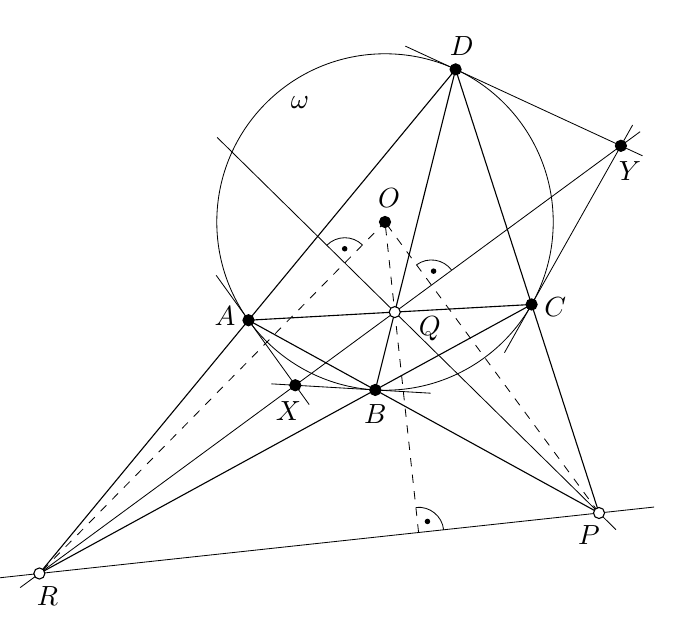
\begin{tikzpicture}[x=1.125cm,y=1.125cm]
		%\clip (-2.49,-1.484) rectangle (5.224,5.035);
		\draw [line width=0.3] (2.11,2.896) coordinate (O) circle (1.899);
		\coordinate (A) at (0.569,1.787);
		\coordinate (B) at (2,1);
		\coordinate (C) at (3.765,1.965);
		\coordinate (D) at (2.907,4.619);
		\coordinate (P) at (4.526,-0.389);
		\coordinate (Q) at (2.22,1.879);
		\coordinate (R) at (-1.792,-1.072);
		\coordinate (X) at (1.097,1.053);
		\coordinate (Y) at (4.773,3.756);
		\coordinate (P1) at (2.634,2.183);
		\coordinate (Q1) at (2.489,-0.609);
		\coordinate (R1) at (1.656,2.434);
		\draw (B) to (D) to (R) to (C) to (P) to (A) to (C) to (D);
		\draw [dash phase=-1.2,line width=0.3,dashed] (O) to (P);
		\draw [line width=0.3,dashed] (Q1) to (O);
		\draw [dash phase=0.4,line width=0.3,dashed] (O) to (R);
		\draw [line width=0.3,shorten <=-2ex,shorten >=-2em] (X) to (A);
		\draw [line width=0.3,shorten <=-2ex,shorten >=-2em] (X) to (B);
		\draw [line width=0.3,shorten <=-2ex,shorten >=-2em] (Y) to (C);
		\draw [line width=0.3,shorten <=-2ex,shorten >=-2em] (Y) to (D);
		\draw [line width=0.3,shorten <=-2em,shorten >=-2em] (P) to (R);
		\draw [line width=0.3,shorten <=-2ex,shorten >=-2ex] (Y) to (R);
		\draw [line width=0.3,shorten <=-2ex,shorten >=-9em] (P) to (Q);
		\draw [line width=0.3,shift={(P1)}] (36.333:0.32cm) arc (36.333:126.333:0.32cm);
		\fill [shift={(P1)}] (81.333:0.18cm) circle (1pt);
		\draw [line width=0.3,shift={(Q1)}] (6.171:0.32cm) arc (6.171:96.171:0.32cm);
		\fill [shift={(Q1)}] (51.171:0.18cm) circle (1pt);
		\draw [line width=0.3,shift={(R1)}] (45.475:0.32cm) arc (45.475:135.475:0.32cm);
		\fill [shift={(R1)}] (90.475:0.18cm) circle (1pt);
		\draw[fill=black] (A) circle (2pt) node[shift={(170:2ex)}] {$A$};
		\draw[fill=black] (B) circle (2pt) node[shift={(270:2ex)}] {$B$};
		\draw[fill=black] (C) circle (2pt) node[shift={(-5:2ex)}] {$C$};
		\draw[fill=black] (D) circle (2pt) node[shift={(75:2ex)}] {$D$};
		\draw[fill=black] (O) circle (2pt) node[shift={(80:2ex)}] {$O$};
		\draw[fill=white] (P) circle (2pt) node[shift={(245:2ex)}] {$P$};
		\draw[fill=white] (Q) circle (2pt) node[shift={(335:3.25ex)}] {$Q$};
		\draw[fill=white] (R) circle (2pt) node[shift={(290:2ex)}] {$R$};
		\draw[fill=black] (X) circle (2pt) node[shift={(255:2.25ex)}] {$X$};
		\draw[fill=black] (Y) circle (2pt) node[shift={(290:2.25ex)}] {$Y$};
		\node at (1.15,4.25) {$\omega$};
	\end{tikzpicture}
\end{figure}

\begin{proof}
	Wir werden nur zeigen, dass $QR$ die Polare von~$P$ ist; die anderen beiden Aussagen sind völlig analog. Aus der Definition der Polaren folgt dann auch sofort $OP\perp QR$.
	
	Sei $X$ der Schnittpunkt der Tangenten an~$\omega$ in $A$~und~$B$ und sei $Y$ der Schnittpunkt der Tangenten an~$\omega$ in $C$~und~$D$. Dann ist $X$ der Pol von~$AB$ und $Y$~der Pol von~$CD$. Weil $P$ der Schnittpunkt von $AB$ und~$CD$ ist, muss nach dem Satz von La~Hire $XY$ die Polare von~$P$ sein. Wir müssen also nur zeigen, dass $Q$~und~$R$ auf~$XY$ liegen. Aus dem Satz von Pascal im entarteten Sehnensechseck $AACBBD$ folgt, dass $X$,~$Q$ und~$R$ kollinear sind (wobei wir die \enquote{Geraden $AA$ und~$BB$} wie üblich als die Tangenten an~$\omega$ in $A$~und~$B$ interpretieren). Analog folgt aus dem Satz von Pascal im entarteten Sehnensechseck $CCADDB$, dass $Y$,~$Q$ und~$R$ kollinear sind.
\end{proof}

Der entscheidende Trick im Beweis war, den Satz von Pascal auf ein entartetes Sehnensechseck anzuwenden. Das ist ganz allgemein ein sehr nützlicher Trick und ihr solltet ihn im Hinterkopf behalten.

An dem folgenden Satz demonstrieren wir ein letztes Mal die Methoden dieses Abschnittes.

\begin{satzmitnamen}[Schmetterlingssatz]
	Sei $ABCD$ ein konvexes Sehnenviereck mit Umkreis~$\omega$. Sei $Q$ der Schnittpunkt der Diagonalen $AC$ und~$BD$. Eine Gerade~$\ell$ durch~$Q$ schneidet den Umkreis~$\omega$ in $X$~und~$Y$ und die Geraden $AB$ und~$CD$ in $K$~und~$L$. Der Punkt~$Q$ ist der Mittelpunkt von~$\overline{XY}$ genau dann, wenn $Q$ der Mittelpunkt von~$\overline{KL}$ ist.
\end{satzmitnamen}

\begin{figure}[ht]
	\centering
	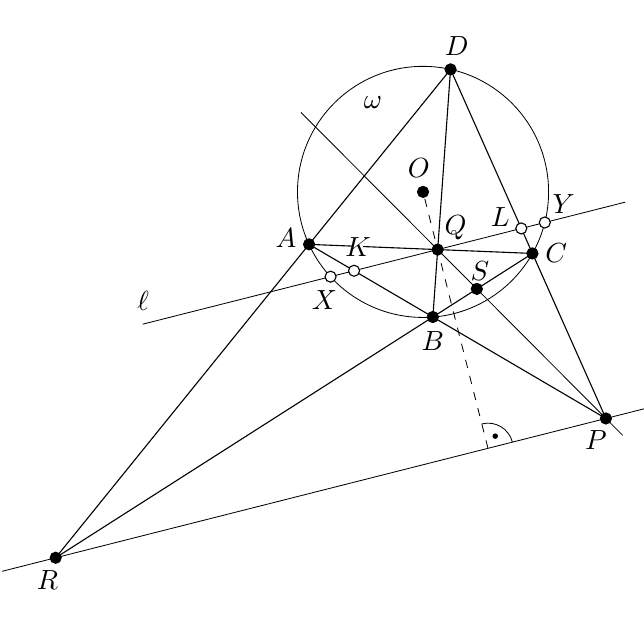
\begin{tikzpicture}[x=0.8cm,y=0.8cm]
		%\clip (-4.945,-3.4) rectangle (5.704,5.518);
		\draw [line width=0.3] (1.844,2.986) coordinate (O) circle (1.993);
		\coordinate (A) at (0.035,2.153);
		\coordinate (B) at (2,1);
		\coordinate (C) at (3.581,2.009);
		\coordinate (D) at (2.281,4.931);
		\coordinate (P) at (4.747,-0.611);
		\coordinate (Q) at (2.076,2.07);
		\coordinate (R) at (-3.988,-2.822);
		\coordinate (S) at (2.698,1.446);
		\coordinate (K) at (0.749,1.734);
		\coordinate (L) at (3.404,2.406);
		\coordinate (X) at (0.376,1.64);
		\coordinate (Y) at (3.777,2.5);
		\coordinate (Q1) at (2.875,-1.085);
		\draw (A) to (B) to (D) to (R) to (C) to (P) to (B) to (C) to (D);
		\draw [shorten >=3.05em] (A) to (Q);
		\draw [shorten <=1.95em] (A) to (C);
		\draw [line width=0.3,dashed] (Q1) to (O);
		\draw [line width=0.3,shorten <=-7em,shorten >=-3em] (X) to (Y);
		\draw [line width=0.3,shorten <=-2em,shorten >=-2em] (P) to (R);
		\draw [line width=0.3,shorten <=-2ex,shorten >=-7em] (P) to (Q);
		\draw [line width=0.3,shift={(Q1)}] (14.201:0.32cm) arc (14.201:104.201:0.32cm);
		\fill [shift={(Q1)}] (59.201:0.18cm) circle (1pt);
		\draw[fill=black] (A) circle (2pt) node[shift={(165:2ex)}] {$A$};
		\draw[fill=black] (B) circle (2pt) node[shift={(270:2ex)}] {$B$};
		\draw[fill=black] (C) circle (2pt) node[shift={(0:2ex)}] {$C$};
		\draw[fill=black] (D) circle (2pt) node[shift={(75:2ex)}] {$D$};
		\draw[fill=black] (O) circle (2pt) node[shift={(100:2ex)}] {$O$};
		\draw[fill=black] (P) circle (2pt) node[shift={(245:2ex)}] {$P$};
		\draw[fill=black] (Q) circle (2pt) node[shift={(50:2.35ex)}] {$Q$};
		\draw[fill=black] (R) circle (2pt) node[shift={(250:2ex)}] {$R$};
		\draw[fill=black] (S) circle (2pt) node[shift={(80:1.5ex)}] {$S$};
		\draw[fill=white] (K) circle (2pt) node[shift={(80:2ex)}] {$K$};
		\draw[fill=white] (L) circle (2pt) node[shift={(152:2ex)}] {$L$};
		\draw[fill=white] (X) circle (2pt) node[shift={(255:2ex)}] {$X$};
		\draw[fill=white] (Y) circle (2pt) node[shift={(45:2.25ex)}] {$Y$};
		\node at (1.05,4.4) {$\omega$};
		\node at (-2.6,1.25) {$\ell$};
	\end{tikzpicture}
\end{figure}

\begin{proof}
	Wir betrachten den Schnittpunkt~$P$ von $AB$ und~$CD$ sowie den Schnittpunkt~$R$ von $AD$ und~$BC$. Außerdem sei $O$ der Umkreismittelpunkt von $ABCD$. Nach dem Satz von Brocard steht $OQ$ senkrecht auf~$RP$. Andererseits ist $Q$ der Mittelpunkt von~$\overline{XY}$ genau dann, wenn $OQ$ auch auf~$XY$ senkrecht steht. Diese Bedingung ist folglich äquivalent zu $RP\parallel XY$.
	
	Sei $S$ der Schnittpunkt von $PQ$ und~$BC$. Nach dem Satz vom vollständigen Vierseit sind $(B,C)$ und $(R,S)$ harmonische Punktepaare. Die Projektion $\pi_P\colon BC\to XY$ durch~$P$ ist eine projektive Abbildung. Also sind auch sind $(K,L)$ und $(Q,T)$ harmonische Punktepaare, wobei $T$ der Schnittpunkt von $RP$ und~$XY$ ist. Somit ist $Q$ genau dann der Mittelpunkt von~$\overline{KL}$, wenn $T=\infty_{XY}$ der unendlich ferne Punkt auf der Geraden~$XY$ ist~-- mit anderen Worten, wenn $RP\parallel XY$. Das zeigt die Behauptung.
\end{proof}

\subsection*{Dualität}
Ein beherrschendes Prinzip in der projektiven Geometrie ist das \emph{Dualitätsprinzip}.

\begin{satzmitnamen}[Dualitätsprinzip]
	Eine geometrische Aussage sollte auch dann noch wahr sein, wenn die Rollen von Punkten und Geraden vertauscht werden, das heißt, wenn die Begriffe \enquote{Punkt} und \enquote{Gerade} sowie \enquote{Schnittpunkt} und \enquote{Verbindungsgerade} vertauscht werden.
\end{satzmitnamen}

Ihr solltet das Dualitätsprinzip nicht allzu wörtlich nehmen. Zum Beispiel ist ja überhaupt nicht klar, was mit Kreisen oder Winkeln passieren soll, wenn Punkte und Geraden vertauscht werden. Solange aber in einer geometrischen Aussage nur Punkte und Geraden vorkommen, ist das Dualitätsprinzip wortwörtlich wahr~-- dank dem Satz von La~Hire! Wenn wir nämlich eine Aussage~$\mathcal A$ bereits bewiesen haben und versuchen, ihre \enquote{duale} Aussage~$\overline{\mathcal A}$ zu beweisen, können wir einen beliebigen Kreis~$\omega$ wählen und alle Punkte durch ihre Polaren sowie alle Geraden durch ihre Pole bezüglich~$\omega$ ersetzen. Dadurch erhalten wir eine äquivalente Aussage. Nach dem Satz von La~Hire ist diese äquivalente Aussage aber genau~$\mathcal A$, was wir schon bewiesen haben.

Ein interessantes Beispiel hierfür ist der Satz von Desargues, der gelegentlich in Olympiadeaufgaben zur Anwendung kommt: Er ist zu seiner eigenen Umkehrung dual! Insbesondere haben wir, sobald wir den Satz bewiesen haben, auch seine Umkehrung bewiesen.

\begin{satzmitnamen}[Satz von Desargues]
	Seien $ABC$ und $A'B'C'$ zwei Dreiecke, sodass sich die Geraden $AA'$, $BB'$ und~$CC'$ in einem Punkt~$Z$ schneiden. Sei $P$ der Schnittpunkt von $BC$ und~$B'C'$, $Q$~der Schnittpunkt von $CA$ und~$C'A'$ sowie $R$~der Schnittpunkt von $AB$ und~$A'B'$. Dann sind $P$,~$Q$ und~$R$ kollinear.
\end{satzmitnamen}

\begin{figure}[ht]
	\centering
	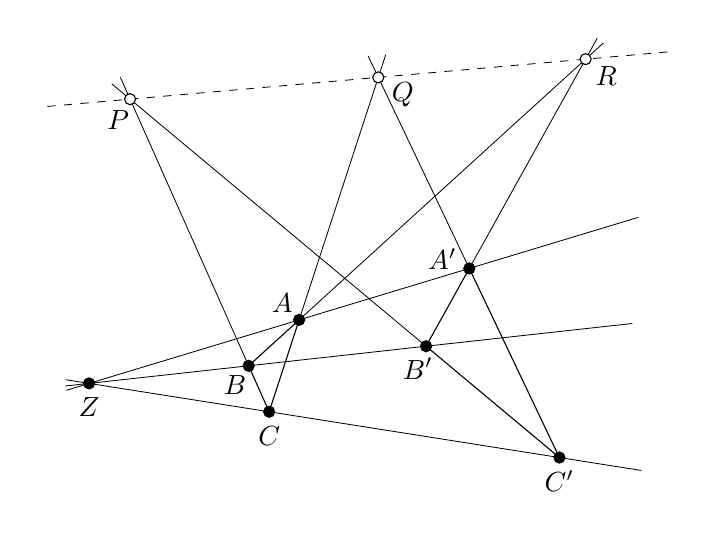
\begin{tikzpicture}[x=0.65cm,y=0.65cm]
		\clip (-7.753,-3.27) rectangle (5.15,6.1);
		\coordinate (A) at (-2.449,0.391);
		\coordinate (B) at (-3.435,-0.507);
		\coordinate (C) at (-3.035,-1.405);
		\coordinate (A1) at (0.876,1.396);
		\coordinate (B1) at (0.031,-0.124);
		\coordinate (C1) at (2.636,-2.299);
		\coordinate (U) at (-5.752,4.703);
		\coordinate (V) at (-0.902,5.129);
		\coordinate (W) at (3.148,5.485);
		\coordinate (Z) at (-6.553,-0.85);
		\draw (A) to (B) to (C) to cycle;
		\draw (A1) to (B1) to (C1) to cycle;
		\draw [line width=0.3,shorten <=-2ex,shorten >=-6.375em] (Z) to (A1);
		\draw [line width=0.3,shorten <=-2ex,shorten >=-7.5em] (Z) to (B1);
		\draw [line width=0.3,shorten <=-2ex,shorten >=-3em] (Z) to (C1);
		\draw [line width=0.3,shorten <=-2ex] (U) to (B);
		\draw [line width=0.3,shorten <=-2ex] (U) to (B1);
		\draw [line width=0.3,shorten <=-2ex] (V) to (A);
		\draw [line width=0.3,shorten <=-2ex] (V) to (A1);
		\draw [line width=0.3,shorten <=-2ex] (W) to (A);
		\draw [line width=0.3,shorten <=-2ex] (W) to (A1);
		\draw[dashed,line width=0.3,shorten <=-3em,shorten >=-3em] (U) to (W);
		\draw[fill=black] (A) circle (2pt) node[shift={(135:2ex)}] {$A$};
		\draw[fill=black] (B) circle (2pt) node[shift={(235:2ex)}] {$B$};
		\draw[fill=black] (C) circle (2pt) node[shift={(270:2ex)}] {$C$};
		\draw[fill=black] (A1) circle (2pt) node[shift={(160:2.4ex)}] {$A'$};
		\draw[fill=black] (B1) circle (2pt) node[shift={(250:2ex)}] {$B'$};
		\draw[fill=black] (C1) circle (2pt) node[shift={(270:2ex)}] {$C'$};
		\draw[fill=white] (U) circle (2pt) node[shift={(240:2ex)}] {$P$};
		\draw[fill=white] (V) circle (2pt) node[shift={(325:2.5ex)}] {$Q$};
		\draw[fill=white] (W) circle (2pt) node[shift={(320:2.25ex)}] {$R$};
		\draw[fill=black] (Z) circle (2pt) node[shift={(270:2ex)}] {$Z$};
	\end{tikzpicture}
\end{figure}

\begin{proof}
	Der Beweis ist sehr ähnlich zum Satz von Pascal. Sei $R'$ der Schnittpunkt von~$AB$ mit~$PQ$ und sei $R''$ der Schnittpunkt von~$A'B'$ mit~$PQ$. Es genügt, $R'=R''$ zu zeigen. Dazu betrachten wir die Projektionen $\pi_A\colon PQ\to BC$, $\pi_Z\colon BC\to B'C'$ und $\pi_{A'}\colon B'C'\to PQ$ durch $A$,~$Z$ und~$A'$. Sei $S$ der Schnittpunkt von $AA'$ und~$PQ$. Weil die Abbildungen $\pi_A$,~$\pi_Z$ und~$\pi_{A'}$ das Doppelverhältnis erhalten, können wir wie folgt umformen:
	\begin{equation*}
		(P,Q;S,R')\overset{\raisebox{0.5ex}{$\scriptstyle\pi_A$}}{=} (P,C;AA'\cap BC,B)\overset{\raisebox{0.5ex}{$\scriptstyle\pi_Z$}}{=} (P,C';AA'\cap B'C',B')\overset{\raisebox{0.5ex}{$\scriptstyle\pi_{A'}$}}{=} (P,Q;S,R'')\,.
	\end{equation*}
	(hierbei bezeichnen $AA'\cap BC$ und $AA'\cap B'C'$ die Schnittpunkte von~$AA'$ mit $BC$ und~$B'C'$). Für jede reelle Zahl $\lambda\neq 0,1$ gibt es aber genau einen Punkt~$Y_\lambda$ auf~$PQ$, für den $(P,Q;S,Y_\lambda)=\lambda$ gilt. Also muss $R'=R''$ gelten und wir sind fertig.
\end{proof}

Gelegentlich lassen sich auch Aussagen dualisieren, die Kreise beinhalten. Ein gutes Beispiel ist der Satz von Pascal: Er ist eine Aussage über sechs Punkte auf einem Kreis, also sollte der duale Satz eine Aussage über sechs \enquote{Geraden auf einem Kreis}, sprich sechs Tangenten sein. Im Satz von Pascal sind die Schnittpunkte der gegenüberliegenden Verbindungsgeraden kollinear. Im dualen Satz sollten dann die Verbindungsgeraden der gegenüberliegenden Schnittpunkte kopunktal sein. Und tatsächlich erhalten wir so einen bekannten Satz:
\begin{satzmitnamen}[Satz von Brianchon]
	Sei $ABCDEF$ ein Tangentensechseck \embrace{das auch überschlagen sein darf}. Dann schneiden sich die Hauptdiagonalen $AD$, $BE$ und~$CF$ in einem Punkt.
\end{satzmitnamen}

Den Satz von Brianchon kennt ihr vielleicht schon aus dem Kapitel \emph{Potenzgeraden} im Heft für Klasse~10 (allerdings haben wir ihn dort nur für nicht-überschlagene Tangentensechsecke bewiesen). Ihr sollt ihn nun mit den Methoden der projektiven Geometrie noch einmal beweisen.

\begin{aufgabe*}
	Beweise den Satz von Brianchon! (\emph{Tipp: Benutze Polaren, um die Aussage auf den Satz von Pascal zurückzuführen.})
\end{aufgabe*}

Wie der Satz von Pascal ist auch der Satz von Brianchon insbesondere dann nützlich, wenn er in entarteten Fällen angewendet wird.

\begin{aufgabe*}
	Sei $ABCD$ ein Tangentenviereck und seien $W$,~$X$, $Y$ und~$Z$ die Berührpunkte des Inkreises mit den Seiten $\overline{AB}$, $\overline{BC}$, $\overline{CD}$ und~$\overline{DA}$.
	\begin{enumerate}
		\item Beweise, dass sich die Geraden $WY$ und~$XZ$ sowie die Diagonalen $AC$ und~$BD$ in einem Punkt~$S$ schneiden.
		\item Beweise, dass sich die Geraden $AX$ und~$CW$ auf~$BD$ schneiden.
		\item Beweise, dass sich die Geraden $AC$, $WX$ und~$YZ$ in einem Punkt~$T$ schneiden. Zeige außerdem, dass $(A,C)$ und $(S,T)$ harmonische Punktepaare sind.
	\end{enumerate}
\end{aufgabe*}

Nachdem wir nun die duale Aussage zum Satz von Pascal ermittelt haben, drängt sich die Frage auf, was denn die duale Aussage zum Satz von Pappos ist. Eine solche duale Aussage muss auf jeden Fall existieren, weil im Satz von Pappos ja nur Punkte und Geraden vorkommen. Statt euch die Antwort direkt zu verraten, werden wir den dualen Satz von Pappos benutzen, um eine Aufgabe von der IMO 2019 zu lösen.

\begin{aufgabe*}[*]
	Im Dreieck $ABC$ liegt ein Punkt~$B_1$ auf der Seite~$\overline{CA}$ und ein Punkt~$C_1$ auf der Seite~$\overline{AB}$. Auf den Strecken $\overline{BB_1}$ und~$\overline{CC_1}$ werden Punkte $P$~und~$Q$ gewählt, sodass $PQ$ parallel zu~$BC$ ist. Ferner sei $P_1$ ein Punkt auf der Verlängerung von~$PC_1$ über~$C_1$ hinaus, für den $\winkel PP_1A=\winkel CBA$ gilt, und sei $Q_1$ ein Punkt auf der Verlängerung von~$QB_1$ über~$B_1$ hinaus, für den $\winkel AQ_1Q=\winkel ACB$ gilt. Beweise, dass $PQQ_1P_1$ ein Sehnenviereck ist.
\end{aufgabe*}

\begin{figure}[ht]
	\centering
	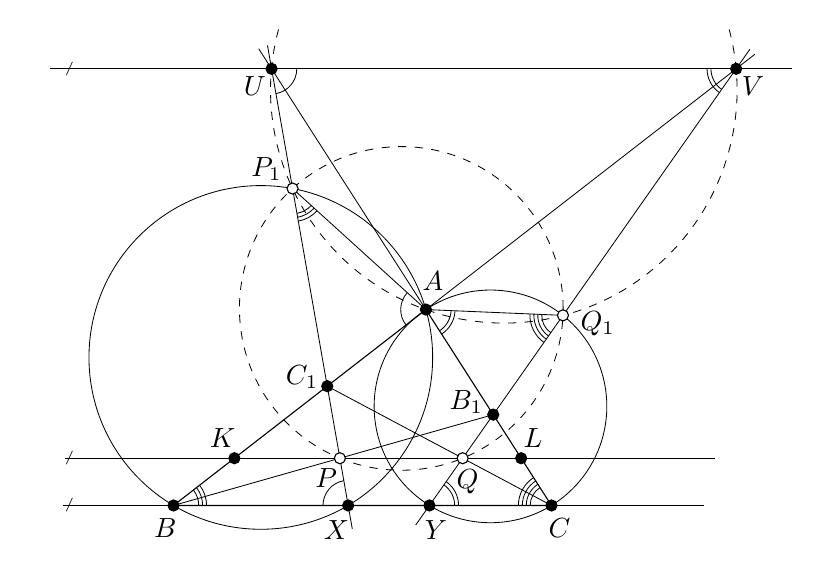
\begin{tikzpicture}[x=0.8cm,y=0.8cm]
		\clip (-4.315,-0.601) rectangle (7.919,7.585);
		\draw [line width=0.3] (-0.614,2.35) circle (2.728);
		\draw [line width=0.3] (3.032,1.573) circle (1.847);
		\draw [dashed,line width=0.3] (1.616,3.128) circle (2.569);
		\draw [dashed,line width=0.3, shift={(3.244,6.599)}] (165:3.703) arc (165:375:3.703);
		\coordinate (A) at (2.007,3.11);
		\coordinate (B) at (-2,0);
		\coordinate (B1) at (3.076,1.442);
		\coordinate (C) at (4,0);
		\coordinate (C1) at (0.441,1.894);
		\coordinate (X) at (0.773,0);
		\coordinate (Y) at (2.063,0);
		\coordinate (P) at (0.641,0.75);
		\coordinate (Q) at (2.59,0.75);
		\coordinate (P1) at (-0.11,5.031);
		\coordinate (Q1) at (4.183,3.018);
		\coordinate (U) at (-0.443,6.932);
		\coordinate (V) at (6.932,6.932);
		\coordinate (K) at (-1.033,0.75);
		\coordinate (L) at (3.519,0.75);
		\draw (A) to (B) to (C) to cycle;
		\draw [line width=0.3] (B) to (B1);
		\draw [line width=0.3] (C) to (C1);
		\draw [line width=0.3, shorten <=-2ex,shorten >=-2ex] (X) to (U);
		\draw [line width=0.3, shorten <=-2ex,shorten >=-2ex] (Y) to (V);
		\draw [line width=0.3] (P1) to (A) to (Q1);
		\draw [line width=0.3, shorten <=-6.125em,shorten >=-7em] (K) to  node[pos=-0.575] {$\scriptscriptstyle/$} (L);
		\draw [line width=0.3, shorten <=-8em,shorten >=-2em] (U) to  node[pos=-0.435] {$\scriptscriptstyle/$} (V);
		\draw [line width=0.3,shorten >=-2ex] (A) to (U);
		\draw [line width=0.3,shorten >=-2ex] (A) to (V);
		\draw [line width=0.3, shorten <=-4em,shorten >=-5.5em] (B) to node[pos=-0.275] {$\scriptscriptstyle/$} (C);
		\draw [line width=0.3,shift={(X)}] (99.951:0.32cm) arc (99.951:180:0.32cm);
		\draw [line width=0.3,shift={(U)}] (-80.049:0.32cm) arc (-80.049:0:0.32cm);
		\draw [line width=0.3,shift={(A)}] (137.765:0.32cm) arc (137.765:217.814:0.32cm);
		\draw [line width=0.3,shift={(Y)}] (0:0.32cm) arc (0:54.917:0.32cm);
		\draw [line width=0.3,shift={(Y)}] (0:0.37cm) arc (0:54.917:0.37cm);
		\draw [line width=0.3,shift={(V)}] (180:0.32cm) arc (180:234.917:0.32cm);
		\draw [line width=0.3,shift={(V)}] (180:0.37cm) arc (180:234.917:0.37cm);
		\draw [line width=0.3,shift={(A)}] (302.659:0.32cm) arc (302.659:357.578:0.32cm);
		\draw [line width=0.3,shift={(A)}] (302.659:0.37cm) arc (302.659:357.578:0.37cm);
		\draw [line width=0.3,shift={(B)}] (0:0.32cm) arc (0:37.815:0.32cm);
		\draw [line width=0.3,shift={(B)}] (0:0.37cm) arc (0:37.815:0.37cm);
		\draw [line width=0.3,shift={(B)}] (0:0.42cm) arc (0:37.815:0.42cm);
		\draw [line width=0.3,shift={(P1)}] (279.951:0.32cm) arc (279.951:317.766:0.32cm);
		\draw [line width=0.3,shift={(P1)}] (279.951:0.37cm) arc (279.951:317.766:0.37cm);
		\draw [line width=0.3,shift={(P1)}] (279.951:0.42cm) arc (279.951:317.766:0.42cm);
		\draw [line width=0.3,shift={(C)}] (122.659:0.27cm) arc (122.659:180:0.27cm);
		\draw [line width=0.3,shift={(C)}] (122.659:0.32cm) arc (122.659:180:0.32cm);
		\draw [line width=0.3,shift={(C)}] (122.659:0.37cm) arc (122.659:180:0.37cm);
		\draw [line width=0.3,shift={(C)}] (122.659:0.42cm) arc (122.659:180:0.42cm);
		\draw [line width=0.3,shift={(Q1)}] (177.578:0.27cm) arc (177.578:234.919:0.27cm);
		\draw [line width=0.3,shift={(Q1)}] (177.578:0.32cm) arc (177.578:234.919:0.32cm);
		\draw [line width=0.3,shift={(Q1)}] (177.578:0.37cm) arc (177.578:234.919:0.37cm);
		\draw [line width=0.3,shift={(Q1)}] (177.578:0.42cm) arc (177.578:234.919:0.42cm);
		\draw[fill=black] (A) circle (2pt) node[shift={(76:2.5ex)}] {$A$};
		\draw[fill=black] (B) circle (2pt) node[shift={(250:2ex)}] {$B$};
		\draw[fill=black] (C) circle (2pt) node[shift={(290:2ex)}] {$C$};
		\draw[fill=black] (B1) circle (2pt) node[shift={(155:2.5ex)}] {$B_1$};
		\draw[fill=black] (C1) circle (2pt) node[shift={(160:2.25ex)}] {$C_1$};
		\draw[fill=white] (P) circle (2pt) node[shift={(235:2ex)}] {$P$};
		\draw[fill=white] (Q) circle (2pt) node[shift={(282:2ex)}] {$Q$};
		\draw[fill=white] (P1) circle (2pt) node[shift={(143:2.75ex)}] {$P_1$};
		\draw[fill=white] (Q1) circle (2pt) node[shift={(-14:3ex)}] {$Q_1$};
		\draw[fill=black] (K) circle (2pt) node[shift={(120:2ex)}] {$K$};
		\draw[fill=black] (L) circle (2pt) node[shift={(60:2ex)}] {$L$};
		\draw[fill=black] (U) circle (2pt) node[shift={(225:2ex)}] {$U$};
		\draw[fill=black] (V) circle (2pt) node[shift={(-45:2ex)}] {$V$};
		\draw[fill=black] (X) circle (2pt) node[shift={(244:2.25ex)}] {$X$};
		\draw[fill=black] (Y) circle (2pt) node[shift={(285:2.125ex)}] {$Y$};
	\end{tikzpicture}
\end{figure}

\begin{proof}[Lösung]
	Sei $X$ der Schnittpunkt von $PC_1$ mit~$BC$ und $Y$~der Schnittpunkt von $QB_1$ mit~$BC$. Dann gilt $\winkel XP_1A=\winkel PP_1A=\winkel CBA=\winkel XBA$, also ist $BXAP_1$ ein Sehnenviereck. Analog ist $YCQ_1A$ ein Sehnenviereck. Sei ferner $U$ der Schnittpunkt von $PC_1$ mit~$AC$ und $V$~der Schnittpunkt von $QB_1$ mit~$AB$. Wir lösen die Aufgabe zuerst durch eine einfache Winkeljagd unter der Annahme, dass $UV$ parallel zu $PQ$ und~$BC$ ist. Unter dieser Annahme folgt aus dem Wechselwinkelsatz $\winkel P_1XB=\winkel P_1UV$. Andererseits ist nach Peripheriewinkelsatz $\winkel P_1XB=\winkel P_1AB$. Es folgt $\winkel VAP_1=180^\circ -\winkel P_1AB=180^\circ -\winkel P_1UV$, also ist $P_1AVU$ ein Sehnenviereck. Mit analoger Begründung ist auch $AQ_1VU$ ein Sehnenviereck, sodass die fünf Punkte $P_1$,~$A$, $Q_1$, $V$ und~$U$ auf einem Kreis liegen. Nach dem Stufen- und Nebenwinkelsatz an den Parallelen $PQ$ und~$UV$ gilt nun $\winkel QPP_1=180^\circ-\winkel P_1UV$. Im Sehnenviereck $P_1Q_1VU$ gilt aber $180^\circ-\winkel P_1UV=\winkel VQ_1P_1=180^\circ-\winkel P_1Q_1Q$. Es folgt $\winkel QPP_1=180^\circ-\winkel P_1Q_1Q$ und somit muss $PQQ_1P_1$ in der Tat ein Sehnenviereck sein.
	
	Es bleibt zu zeigen, dass $UV$ wirklich parallel zu $PQ$ und~$BC$ ist. Wenn wir in der projektiven Ebene arbeiten, müssen wir also zeigen, dass sich $UV$, $PQ$ und~$BC$ in einem Punkt schneiden (dieser ist dann zwangsläufig der Schnittpunkt von $BC$ und~$PQ$, also~$\infty_{PQ}$). Und das folgt direkt aus dem dualen Satz von Pappos! Der Satz von Pappos ist nämlich eine Aussage über sechs Punkte, von denen jeweils drei auf einer Geraden liegen. Und hier haben wir es umgekehrt mit sechs Geraden $AB$, $CC_1$, $PP_1$ und $AC$, $BB_1$, $QQ_1$ zu tun, von denen sich jeweils drei in einem Punkt schneiden.
\end{proof}

Statt mit dem dualen Satz von Pappos lässt sich auch direkt über Doppelverhältnisse argumentieren. Dazu führen wir die Schnittpunkte $K$~und~$L$ von~$PQ$ mit $AB$ und~$AC$ ein. Die Projektion $\pi_{B_1}\colon PQ\to AB$ durch~$B_1$ erhält das Doppelverhältnis, also gilt $(P,Q;K,L)=(B,V;K,A)$. Die Projektion $\pi_{C_1}\colon PQ\to CA$ durch~$C_1$ erhält ebenfalls das Doppelverhältnis, also gilt $(P,Q;K,L)=(U,C;A,L)$. Es folgt
\begin{equation*}
	\frac{BK}{KV}\bigg/\frac{BA}{AV}=\frac{UA}{AC}\bigg/\frac{UL}{LC}\,.
\end{equation*}
Weil $KL$ parallel zu~$BC$ ist, folgt aus dem Strahlensatz (der auch für gerichtete Streckenlängen gültig ist) $BK/BA=LC/AC$.
% Tien: Vielleicht willst du zu ungerichteten Streckenlängen übergehen. Oder erwähnst kurz, dass der Strahlensatz so auch für gerichtete Streckenlängen gilt.
Die obige Gleichung impliziert also $AV/KV=UA/UL$. Nach der Umkehrung des Strahlensatzes muss dann $UV$ parallel zu~$KL$ sein.

Hier sehen wir einen letzten Trick in Aktion: Wenn ihr ein Verhältnis von Strecken berechnen müsst --~zum Beispiel, für ein Strahlensatzargument wie oben, oder für Argumente mit den Sätzen von Ceva und Menelaos~-- dann könnt ihr versuchen, dieses Verhältnis zu einem Doppelverhältnis zu ergänzen, das ihr wiederum mithilfe geeigneter Projektionen auf ein Doppelverhältnis zurückführen könnt, welches einfacher zu berechnen ist.

\subsection*{Weitere Übungsaufgaben}
\begin{aufgabe*}
	Einem Dreieck $ABC$ sei ein Halbkreis~$\omega$ so einbeschrieben, dass der Durchmesser~$\overline{EF}$ auf der Seite~$\overline{AB}$ liegt. Dabei befindet sich $E$ zwischen $F$~und~$A$. Der Halbkreis~$\omega$ berühre die Seiten $\overline{BC}$ und~$\overline{CA}$ in $G$~und~$H$. Schließlich sei $S$ der Schnittpunkt von $GE$ und~$FH$ sowie $T$~der Schnittpunkt von $EH$ und~$FG$. Zeige, dass $C$ der Mittelpunkt der Strecke~$\overline{ST}$ ist.
\end{aufgabe*}

\begin{aufgabe*}
	Sei $ABC$ ein Dreieck mit Inkreis~$\omega$. Sei $D$ der Berührpunkt von~$\omega$ mit der Seite~$\overline{BC}$, sei $X$ der von~$D$ verschiedene Schnittpunkt von~$AD$ mit~$\omega$ und seien $Y$,~$Z$ die von~$X$ verschiedenen Schnittpunkte von $BX$,~$CX$ mit~$\omega$. Beweise, dass sich $BZ$ und~$CY$ auf~$AD$ schneiden.
\end{aufgabe*}

\begin{aufgabe*}[*]
	Sei $ABC$ ein Dreieck mit Inkreis~$\omega$ und Inkreismittelpunkt~$I$. Seien $D$,~$E$ und~$F$ die Berührpunkte von~$\omega$ mit den Seite $\overline{BC}$, $\overline{CA}$ und~$\overline{AB}$. Schließlich sei $M$ der Mittelpunkt von~$\overline{BC}$. Beweise, dass sich die Geraden $AM$, $DI$ und~$EF$ in einem Punkt schneiden.
\end{aufgabe*}

\begin{aufgabe*}[*]
	Die Punkte $A$,~$B$, $C$ und~$D$ liegen in dieser Reihenfolge auf einem Kreis~$\omega$ mit Mittelpunkt~$O$. Sei $K$ der Schnittpunkt von $AC$ und~$BD$. Ein weiterer Kreis~$\omega_1$ mit Mittelpunkt auf der Strecke~$\overline{OK}$ schneide die Strecken $\overline{AB}$ und~$\overline{CD}$ in den Punkten $A_1$~und~$B_1$ bzw.\ $C_1$~und~$D_1$. Angenommen, $K$~liegt auf der Geraden~$A_1C_1$ und es gilt $\abs*{A_1K}\neq \abs*{KC_1}$. 
	% Tien: Gibt es einen bestimmten Grund, warum A_1K und KC_1 gerichtete Streckenlängen sind? Ansonsten finde ich, dass sich Betragsstriche besser lesen lassen.
	Beweise, dass $K$ dann auch auf~$B_1D_1$ liegt.
\end{aufgabe*}

\begin{aufgabe*}[*]
	Sei $ABCD$ ein konvexes Sehnenviereck. Sei $K$ der Schnittpunkt der Diagonalen $AC$ und~$BD$. Die Mittelpunkte von $\overline{AC}$ und~$\overline{BD}$ bezeichnen wir mit $M$~und~$N$. Die Umkreise $\odot ABM$ und $\odot CDM$ schneiden sich außer in~$M$ noch in~$L$. Zeige, dass $KLMN$ ein Sehnenviereck ist.
\end{aufgabe*}

\begin{aufgabe*}[*]
	Sei $ABCD$ ein konvexes Viereck, sodass die Diagonale~$BD$ zugleich auch die Winkelhalbierende von $\winkel CBA$ ist. Der Umkreis $\odot ABC$ schneide die Strecken $\overline{CD}$ und~$\overline{DA}$ in den inneren Punkten $P$~und~$Q$. Die Parallele zu~$AC$ durch~$D$ scheide die Geraden $BA$ und~$BC$ in den Punkten $R$~und~$S$. Zeige, dass die vier Punkte $P$,~$Q$, $R$ und~$S$ auf einem Kreis liegen.
\end{aufgabe*}

\begin{aufgabe*}[*]
	In einem gleichschenkligen Dreieck $ABC$ mit $\abs{AB}=\abs{AC}$ sei $M$ der Mittelpunkt der Seite~$\overline{BC}$. Weiter sei $P$ ein Punkt auf der Parallelen zu~$BC$ durch~$A$, für den $\abs{PB}<\abs{PC}$ gilt. Ferner sei $X$ ein Punkt auf der Verlängerung von~$\overline{PB}$ über~$B$ hinaus und $Y$~ein Punkt auf der Verlängerung von~$\overline{PC}$ über~$C$ hinaus, sodass $\winkel MXP=\winkel PYM$ gilt. Beweise, dass $APXY$ ein Sehnenviereck ist.
\end{aufgabe*}
